\section{Finden von ähnlichen Hotels}
\label{sec:find_similar}
Das finden von ähnlichen Hotels ist die Grundlage dieses Konzeptes. Um dies zu erreichen soll das vorgehen, welches in der Sektion \emph{\nameref{sec:aehnliche_hotels}} beschrieben wurde, verfolgt werden. Angefangen mit der Datenbeschaffung, muss sich zunächst ein überblick darüber gemacht werden, welche Daten schon vorhanden sind und welche Daten gegeben falls noch besorgt werden müssen, bevor dann mit der Datenanalyse und der Modellierung weiter gemacht werden kann. 

\subsection{Datenbeschaffung}
\label{subsec:Datenbeschaffung}
Durch die verschiedenen Property Management Systeme sind für die einzelnen Hotels bereits Stammdaten wie Zimmeranzahl oder Zimmerkategorien vorhanden. Zudem wird der jeweilige Kunde beim Einrichten von happyhotel auch schon nach verschiedenen Daten befragt. Unter den Daten, die bei einem Kunden abgefragt werden, gehören Informationen wie zum Beispiel die Adresse des jeweiligen Hotels. 
\newline
\newline
Werden nun alle schon vorhanden Informationen zusammengetragen, die bisher in der Datenbank zur Verfügung stehen, entsteht dabei das folgende Dataframe:
\begin{figure}[h]
    \centering
    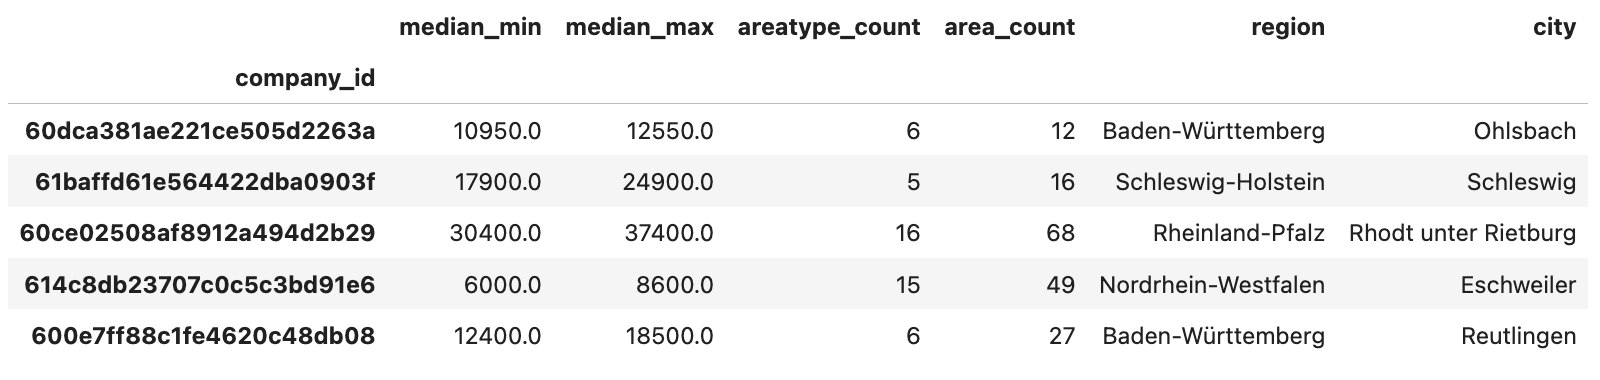
\includegraphics[width=1\textwidth, center]{Features_1.png}
    \caption[Alle schon vorhanden Features]{Alle schon vorhanden Features}
    \label{img:all_Features}
\end{figure}

In Abbildung \ref{img:all_Features} sind die Daten zu sehen, die bislang zur Verfügung stehen, wobei sich die \emph{median\_min} und \emph{median\_max} Werte auf den Median aller Zimmerkategorie-Preise bezieht.
\newline
\newline
Dadurch, dass \emph{region} und \emph{city} manuell vom Kunden eingetragene Werte sind, ergab sich eine gewisse Skepsis, ob alle Werte norm-konform eingetragen wurden. Aufgrund dieser Skepsis sollte eine kleine Datenanalyse getätigt werden. 
\newline
\newline
Bei der Datenanalyse wurde jeweils nach der Region und nach der Stadt gruppiert, um zu prüfen ob die Daten so benutzt werden können. Im Folgenden sind die Werte jeweils für die Region und für die Stadt zu sehen:

\begin{figure}[h]
    \centering
    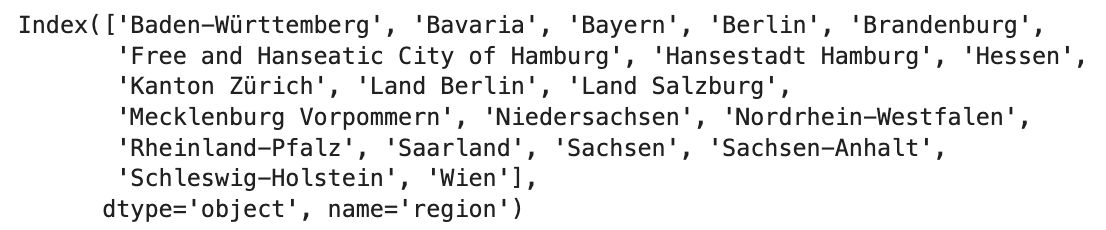
\includegraphics[width=0.8\textwidth, center]{region_1.png}
    \caption[Alle vorhanden Regionen]{Alle vorhanden Regionen}
    \label{img:region_1}
\end{figure}

\begin{figure}[h]
    \centering
    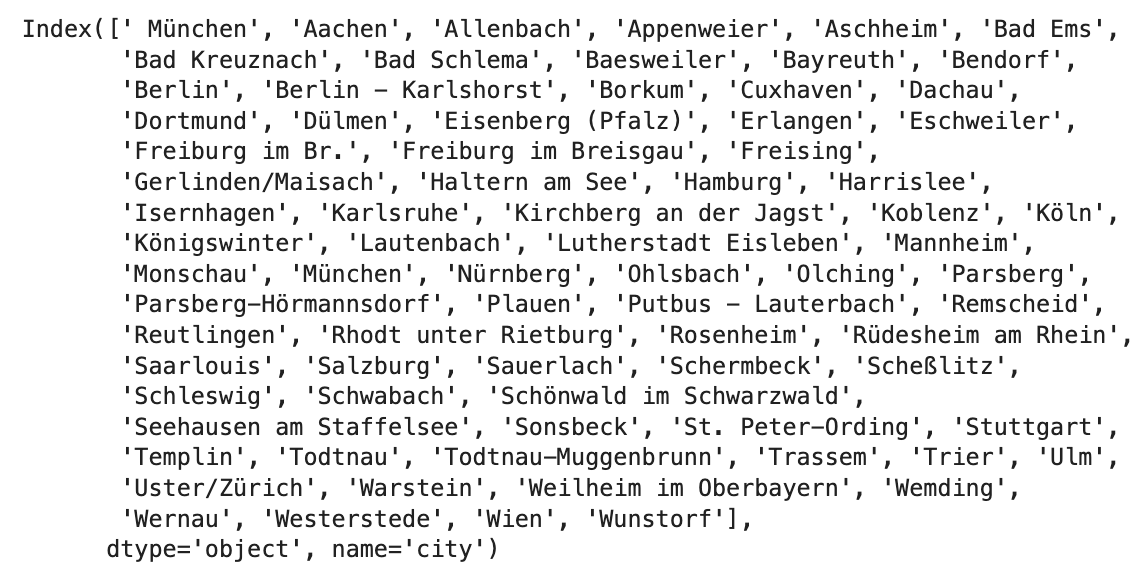
\includegraphics[width=0.8\textwidth, center]{city_1.png}
    \caption[Alle vorhanden Städte]{Alle vorhanden Städte}
    \label{img:city_1}
\end{figure}

Es ist eindeutig zu erkennen, dass es sowohl bei der Region als auch bei der Stadt zu einer Inkonsistenz kommt. So wurde die Region \emph{Berlin} sowohl als \emph{Berlin}, als auch mit \emph{Land Berlin} angegeben. Auch bei der Stadt ist die Diskrepanz deutlich zu erkennen, -so wurde bspw. \emph{München} mit Leerzeichen vorne dran angegeben oder die Stadt Freiburg einmal mit der Abkürzung \emph{Br.} und ein anderes Mal mit komplett ausgeschriebenen \emph{Breisgau} angegeben. Es ergab sich also, dass diese Werte so wie sie sind, nicht verwendet werden können.

\subsubsection{Beschaffung von Region, City und Stadtgröße}
\label{subsubsec:region_city_size}
Durch eine schon im Vorfeld getätigte Arbeit, existiert zu jedem Hotel in unserer Datenbank, die Koordinaten, repräsentiert durch die zwei Werte Long- und Latitude. Mithilfe von diesen zwei Werten sollte ein Skript geschrieben werden um die Region, die Stadt und Größe der Stadt zu beschaffen. 
\newline
\newline
Für das Skript wurde \emph{Nominatim} API verwendet um die einzelnen Werte zu beschaffen. Im folgenden wird das Skript präsentiert:

\begin{lstlisting}[language=Python, label=lst:RS_Demo, caption=Einfaches Recommendation System für Film vorschläge]
    from geopy.geocoders import Nominatim

def get_region_city_size(latitude, longitude):
    geolocator = Nominatim(user_agent="city_size_app")
    location = geolocator.reverse((latitude, longitude), language='de')

    address = location.raw['address']

    if 'city' in address:
      region = address["city"]
      if 'state' in address:
        region = address["state"]
      return {
            "city": address["city"],
            "region": region,
            "size": "Großstadt"
        }
    elif 'town' in address:
        return {
            "city": address["town"],
            "region": address["state"],
            "size": "Kleinstadt"
        }
    elif 'village' in address:
      region = None
      if 'county' in address:
        region = address["county"]
      if 'state' in address:
        region = address["state"]
      return {
            "city": address["village"],
            "region": region,
            "size": "Kleinstadt"
        }
    else:
        return dict()
\end{lstlisting}

Die Funktion \emph{get\_region\_city\_size} nimmt als Parameter die Long- und Latitude Werte und erzeugt dadurch ein \emph{Dictionary} mit den Werten \emph{region}, \emph{city} und \emph{size}.
\subsubsection{Beschaffung von der Hotelart}
\label{subsubsec:hotelart}
Einer der wichtigsten Eigenschaften, die ein Hotel vorweisen kann, ist die Hotelart von dem jeweiligen Hotel. Die Hotelart hängt maßgeblich mit der zur grundlegenden Preisgestaltung ab. Dies ist einfach zu erklären, da Hotels existieren, die eher auf Wellness ausgelegt sind und somit prinzipiell teurer sind als einfache Urlaubshotels. Somit ist die Art eines Hotels essentiell um ähnliche Hotels zu finden. So soll auch für das Modell die Hotelart vorhanden sein. Dieses Feature muss jedoch erst beschafft werden, da diese Information nicht in der Datenbank hinterlegt ist. 
\newline
\newline
Leider ist der Versuch, die Hotelart auf einem automatisiertem Weg zu bekommen, gescheitert und es blieb nichts anderes übrig als die Hotelart eines jedem Hotels manuell herauszufinden. 
\newline
\newline
Nachdem die Hotelart beschaffen wurde, sieht der Feature-Datensatz wie folgt aus:
\begin{figure}[h]
    \centering
    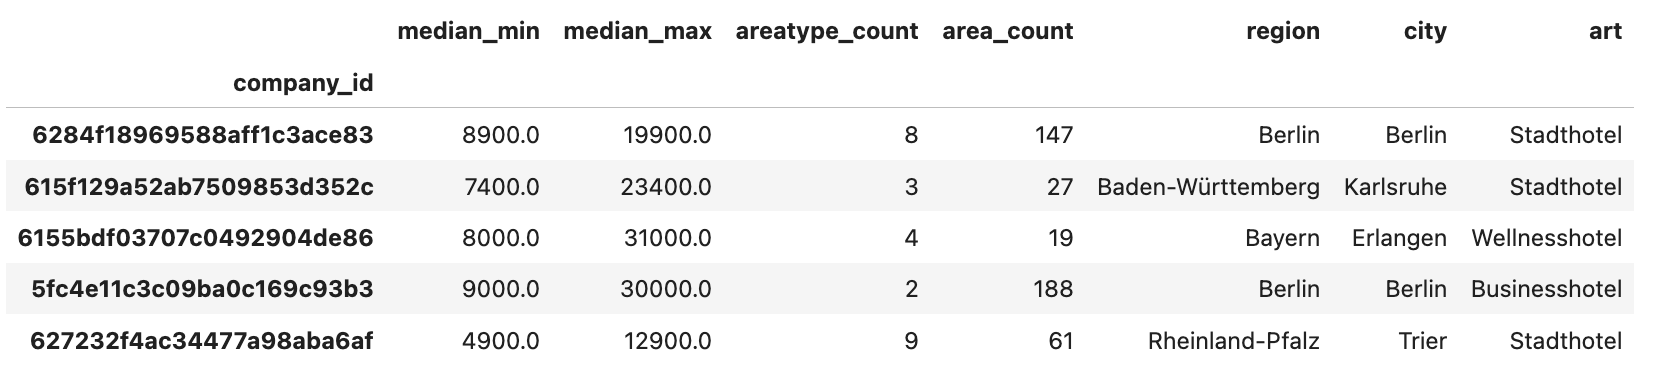
\includegraphics[width=1\textwidth, center]{Features_2.png}
    \caption[Alle schon vorhanden Features #2]{Alle schon vorhanden Features #2}
    \label{img:all_Features_2}
\end{figure}

\subsection{Datenvorverarbeitung}
\label{subsec:Datenvorverarbeitung}
Nach der Datenbeschaffung erfolgt die Datenvorverarbeitung, die darauf abzielt, die Qualität und Integrität der Daten sicherzustellen. Ein zentraler Schwerpunkt liegt dabei auf der Identifikation und Eliminierung fehlerhafter oder ungültiger Datensätze. Häufig wird innerhalb der Datensätze nach Nullwerten gesucht, um diese entweder durch valide Daten zu ersetzen oder in einigen Fällen gänzlich zu entfernen. Im vorliegenden Fall ist es Wichtig, dass sämtliche als verwendbar gekennzeichneten Hotels in die Analyse einbezogen werden. Die Datensätze sollen nicht einfach verworfen werden; vielmehr erfolgt eine gezielte Substitution von Nullwerten durch valide Daten, um eine konsistente und zuverlässige Grundlage für die weiterführende Analyse zu gewährleisten \cite{Agarwal.05.10.2018}.
\newline
\newline
Im folgenden ist die Anzahl aller Nullwerte innerhalb des Datensatzes zu sehen:
\begin{figure}[h]
    \centering
    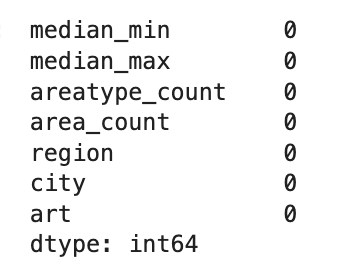
\includegraphics[width=0.4\textwidth, center]{Null_values.png}
    \caption[Summe aller Nullwerte im Datensatz]{Summe aller Nullwerte im Datensatz}
    \label{img:null_values}
\end{figure}

In Abbildung \ref{img:null_values} ist zu sehen, dass innerhalb des es Datensatzes keine Nullwerte gibt und somit auch keine Datenvorverarbeitung getätigt werden muss.
\subsection{Allgemeine Datenanalyse}
\label{subsec:Datenanalyse}
Die Datenanalyse ist ein, wenn nicht sogar der Wichtigste schritt im Data Science Bereich \cite{Agarwal.05.10.2018}. Dabei sollen die Daten ergründet und verstanden werden. Dieser Schritt soll nicht nur ein Verständnis für die vorliegenden Daten schaffen, sondern auch \emph{outlier} erfassen. Meist wird auch versucht innerhalb der Datenanalyse zusammenhänge zu der Zielvariable zu finden. Dies setzt jedoch voraus, dass eine Zielvariable vorhanden ist. In dem vorliegenden Fall existiert keine Zielvariable, da nicht bekannt ist welche Hotels mit welchen Hotels ähnlich sind. Aufgrund dessen, dass keine Zielvariable vorhanden ist, wird die folgende Datenanalyse lediglich dazu genutzt um die Daten besser zu verstehen. Zudem soll festgestellt werden, welche Daten wie als Features verwendet werden können.
\newline
\newline
Für die Datenanalyse soll die Python-Bibliothek \emph{Seaborn} benutzt werden. Die \emph{Seaborn}-Bibliothek stellt ein leistungsstarkes Werkzeug dar, das speziell für die Erstellung von statistischen Grafiken in Python entwickelt wurde \cite{Melanie.2023}. Das Hauptziel besteht darin, die verschiedenen Verteilungen der Features auf anschauliche Weise darzustellen, um einen umfassenden Überblick über die zugrunde liegenden Daten zu ermöglichen. Durch die Nutzung der Funktionalitäten von \emph{Seaborn} wird eine effiziente und ästhetisch ansprechende Visualisierung erreicht, die es ermöglicht, Muster, Ausreißer oder Trends in den Daten leichter zu identifizieren.

\subsubsection{Region Features}
Zuallererst soll ein grober Überblick über die Städte der Hotels innerhalb der Datenbank erstellt werden. Dazu wird innerhalb des Datensatzes nach der Stadt um die Anzahl der Hotels einer Stadt zu ermitteln.

\newpage

\begin{figure}[h]
    \centering
    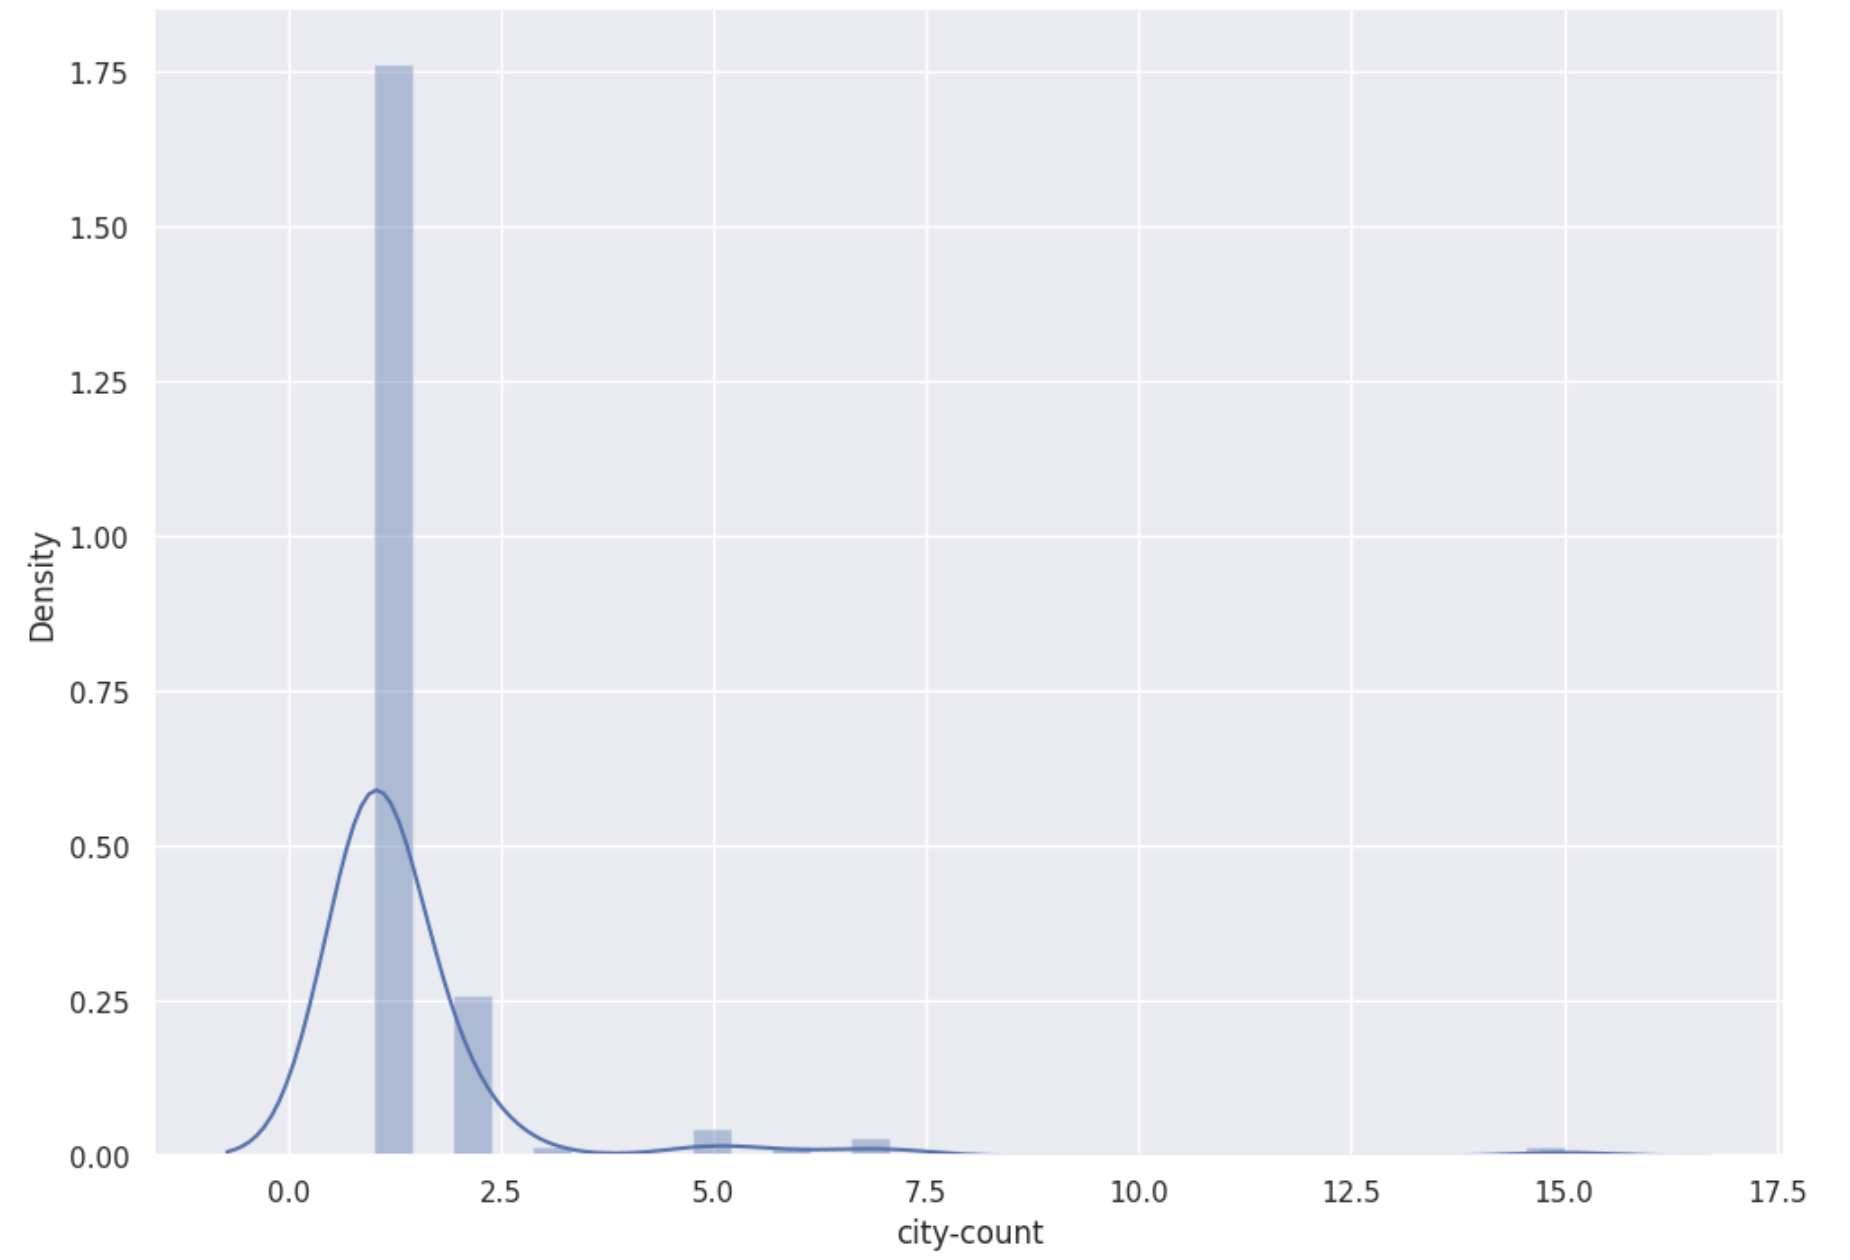
\includegraphics[width=1\textwidth, center]{verteilung_city.png}
    \caption[Verteilung der Städte]{Verteilung der Städte}
    \label{img:verteilung_city}
\end{figure}

Die Analyse der Abbildung \ref{img:verteilung_city} offenbart, dass die überwiegende Mehrheit der in der Datenbank erfassten Städte lediglich über ein einziges Hotel verfügt, welches happyhotel in Anspruch nimmt. Zugleich verdeutlicht die Abbildung \ref{img:verteilung_city}, dass es lediglich einen geringen Anteil von Städten gibt, in denen fünf oder mehr Hotels registriert sind. Dies ist etwas problematisch, da das Feature \emph{City} zu unausgewogen ist und so nicht mit in das Modell gegeben werden kann. Es muss also in einer anderen Form verwendet werden.
\newline
\newline
Momentan werden, wie in der Abbildung \ref{img:all_Features_2} gezeigt, die Stadt und die Region als zwei separate Features aufgelistet. Die Idee ist es nun die zwei Features zu verschmelzen und die Hotels in Regionen aufzuteilen um mehr Informationen zu erhalten. Anstatt also Region und Stadt separat zu haben soll es ein Feature Region geben, welches wie folgt aufgebaut ist: 

\begin{itemize}
    \item Befindet sich innerhalb einer Stadt Fünf oder mehr Hotels, so wird die Stadt ohne jegliche Modifikation als Region genommen.
    \item Befindet sich innerhalb einer Stadt weniger als Fünf Hotels, so setzt sich die Region aus der ursprünglichen Region, also dem Bundesland und der Größe der Stadt zusammen nach dem Schema: {Region}-{Größe}
\end{itemize}

Für die Idee muss zunächst ermittelt werden, in welchen Städte sich Fünf oder mehr Hotels befinden. Auch diese Information kann wie folgt Visualisiert werden:

\begin{figure}[h]
    \centering
    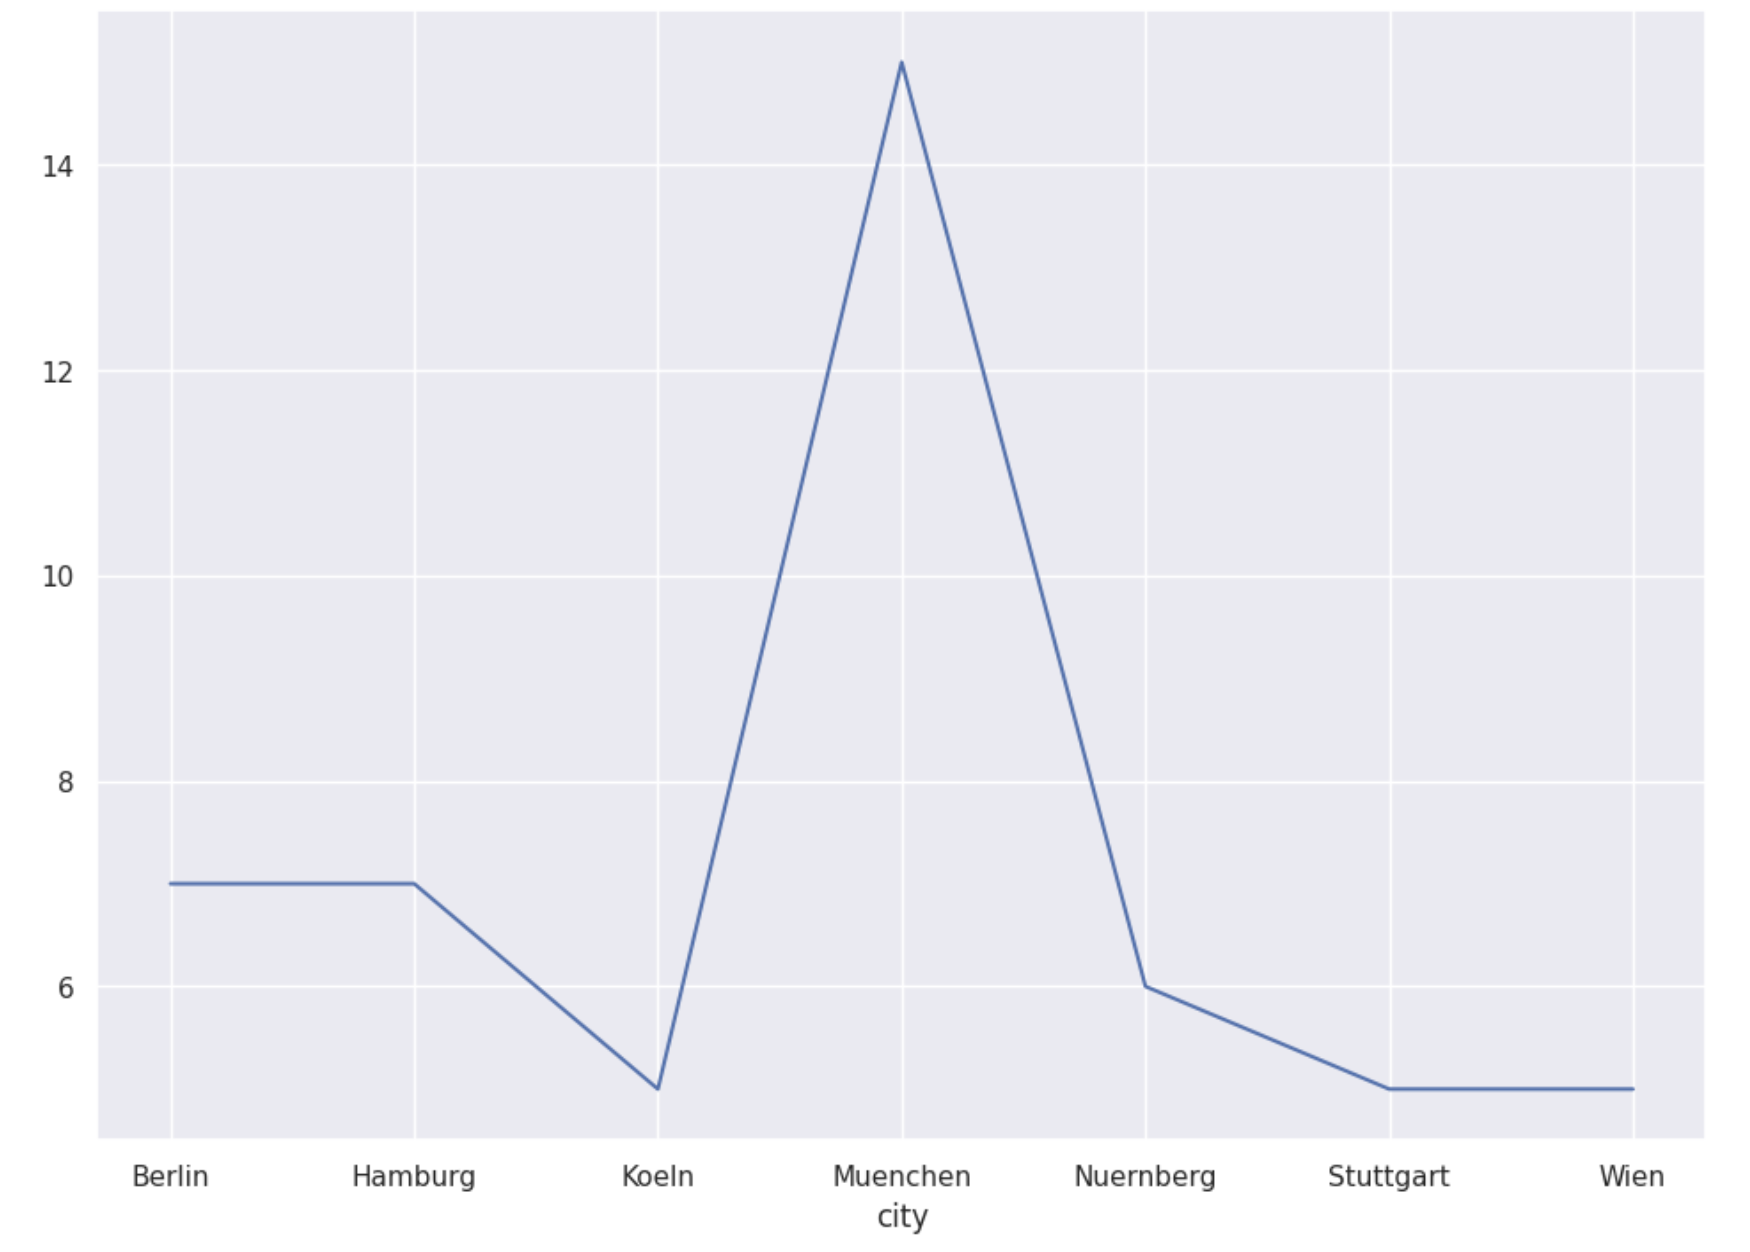
\includegraphics[width=1\textwidth, center]{city_five_or_more.png}
    \caption[Städte mit Fünf oder mehr Hotels]{Städte mit Fünf oder mehr Hotels}
    \label{img:city_five_or_more}
\end{figure}

Ganz klar zu erkennen ist, dass die Sieben Städte Berlin, Hamburg, Köln, München, Nürnberg, Stuttgart, und Wien die Städte sind, in denen Fünf oder mehr Hotels vorhanden sind. Die aufgelisteten Städte können dementsprechend so übernommen werden und für alle anderen wird die Regel von oben angewandt.
\newline
Nach der Umformulierung von Region und Stadt sieht der Datensatz wie folgt aus:

\begin{figure}[h]
    \centering
    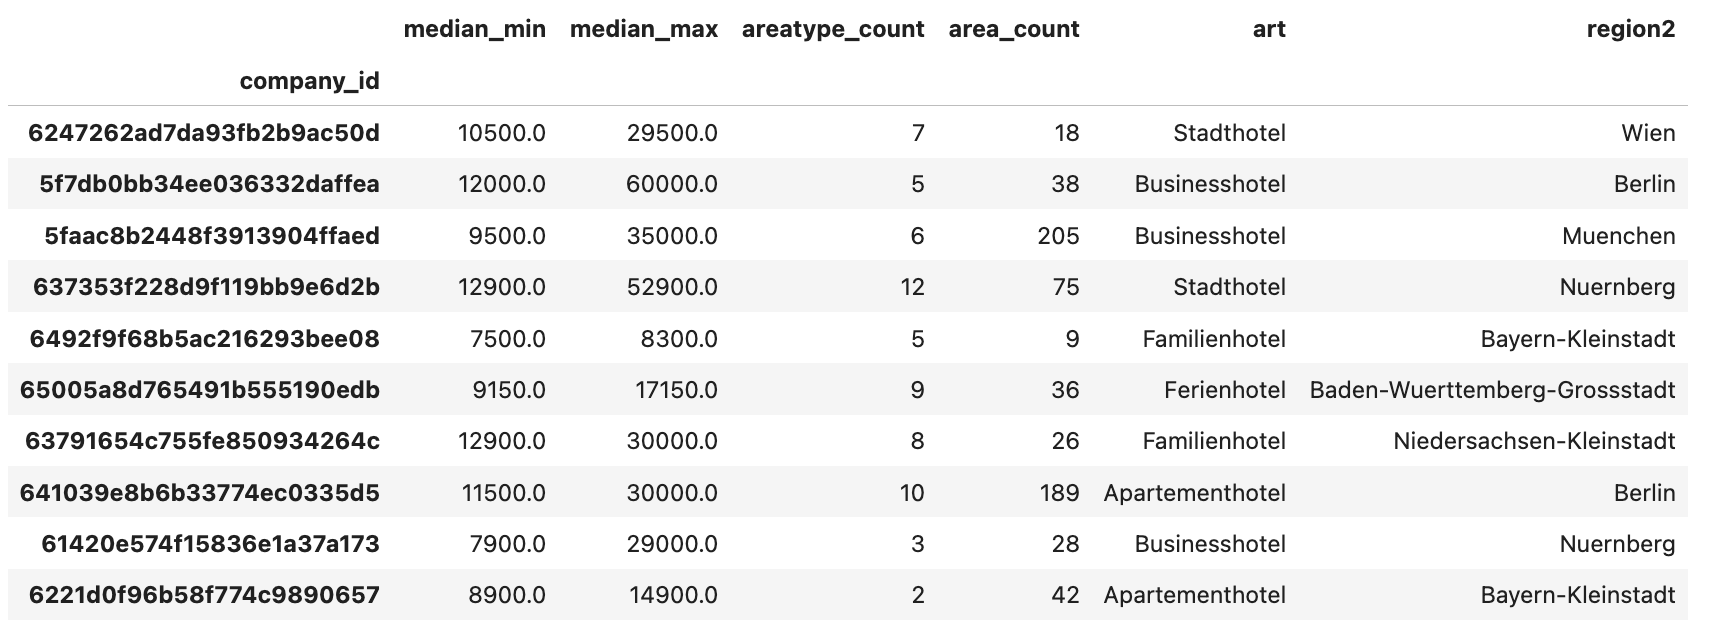
\includegraphics[width=1\textwidth, center]{all_features_3.png}
    \caption[Datensatz nach der Umformulierung]{Datensatz nach der Umformulierung}
    \label{img:all_features_3}
\end{figure}

Auch hier soll wieder die Verteilung visualisiert werden

\begin{figure}[h]
    \centering
    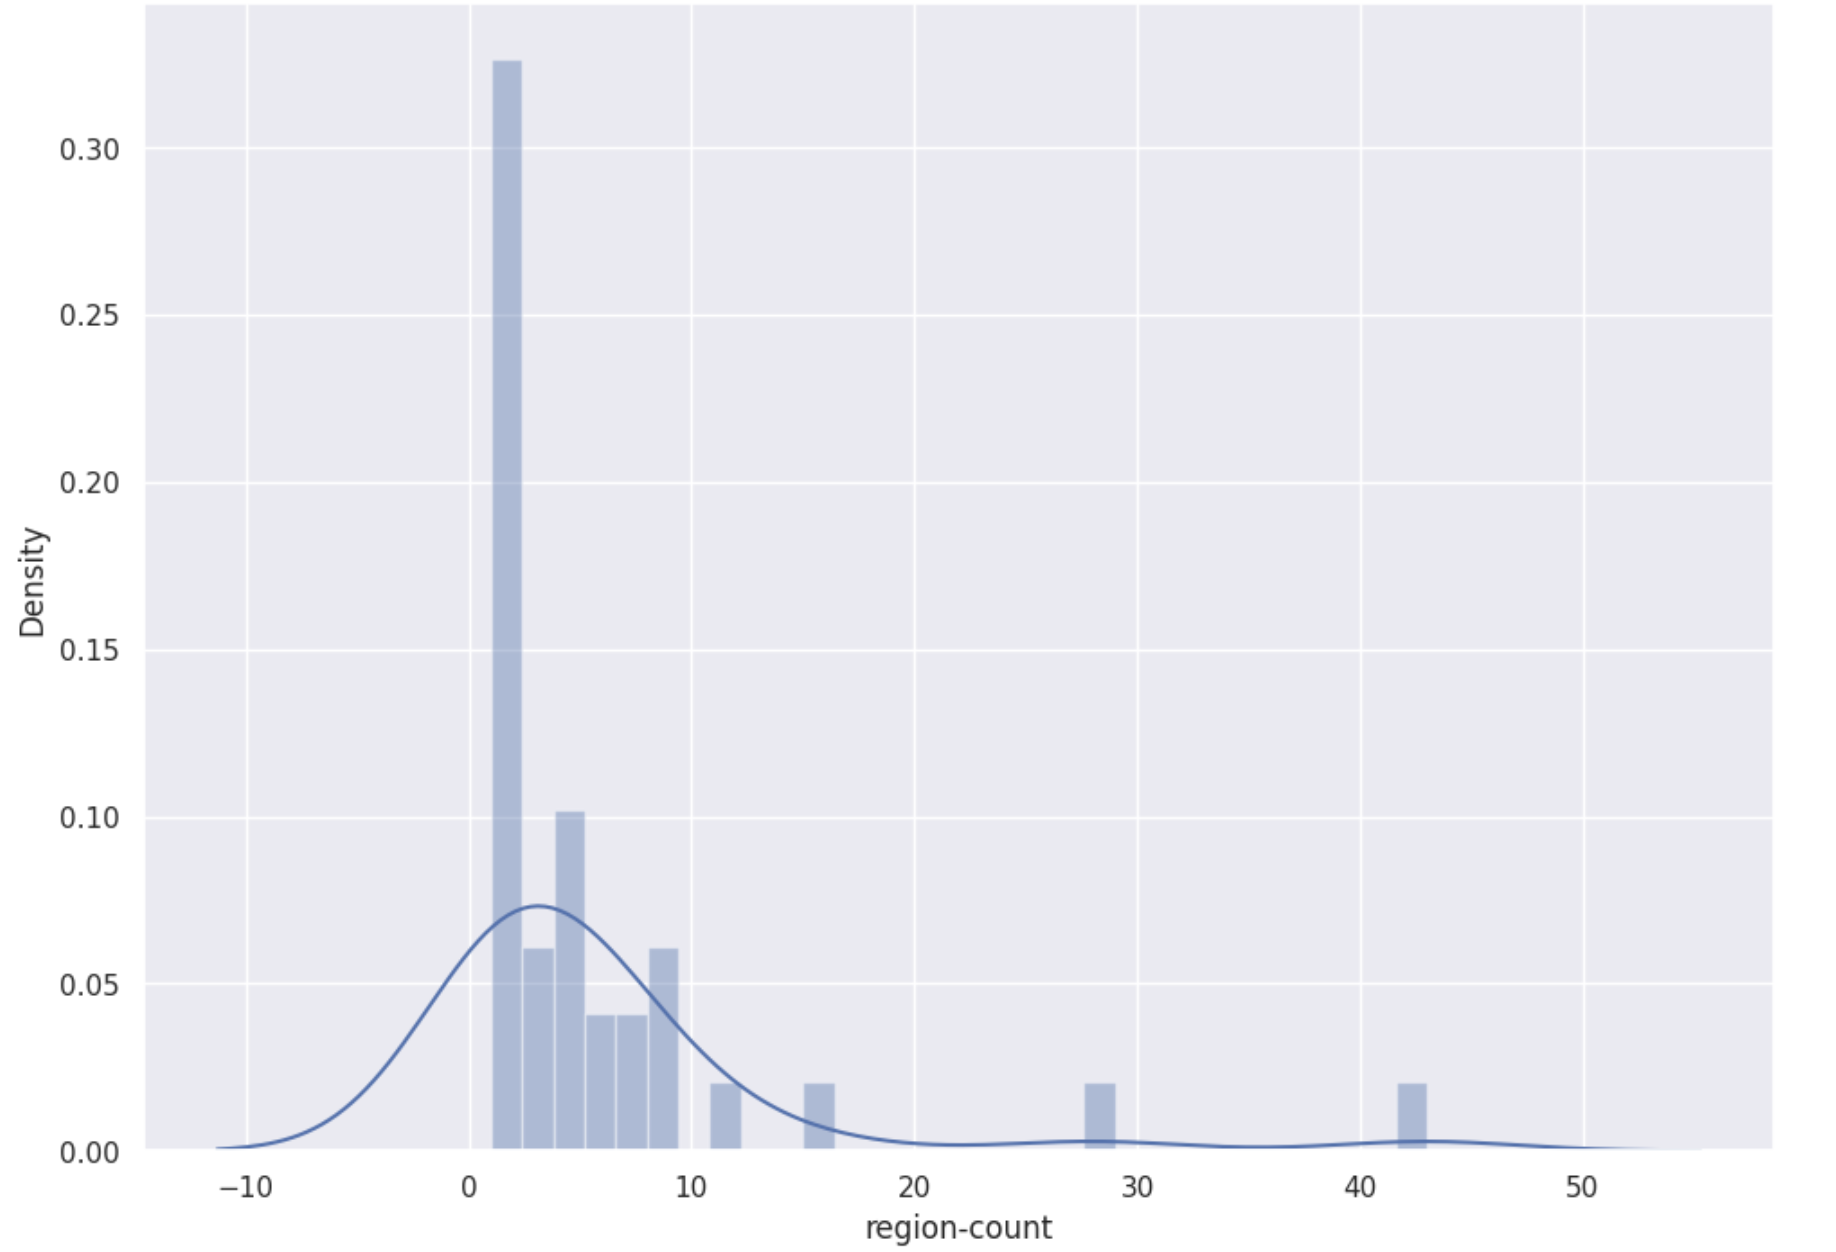
\includegraphics[width=1\textwidth, center]{verteilung_region2.png}
    \caption[Verteilung des neuen Features \emph{region2}]{Verteilung des neuen Features \emph{region2}}
    \label{img:verteilung_region_2}
\end{figure}

Es zeigt sich, dass noch immer ein großer Anteil des Datensatzes niedrigeren Bereich sich befindet, jedoch konnte mit der Modifikation ein bisschen mehr Varianz in die Daten gebracht werden.

\subsubsection{Preis Features}
Als nächstes sollen die Preis Features, namentlich betitelt mit \emph{median\_min} und \emph{median\_max}, erkundet und visualisiert werden. Hierzu soll wie auch bei der Region zunächst die Verteilung betrachtet werden:
\newpage
\begin{figure}[h]
    \centering
    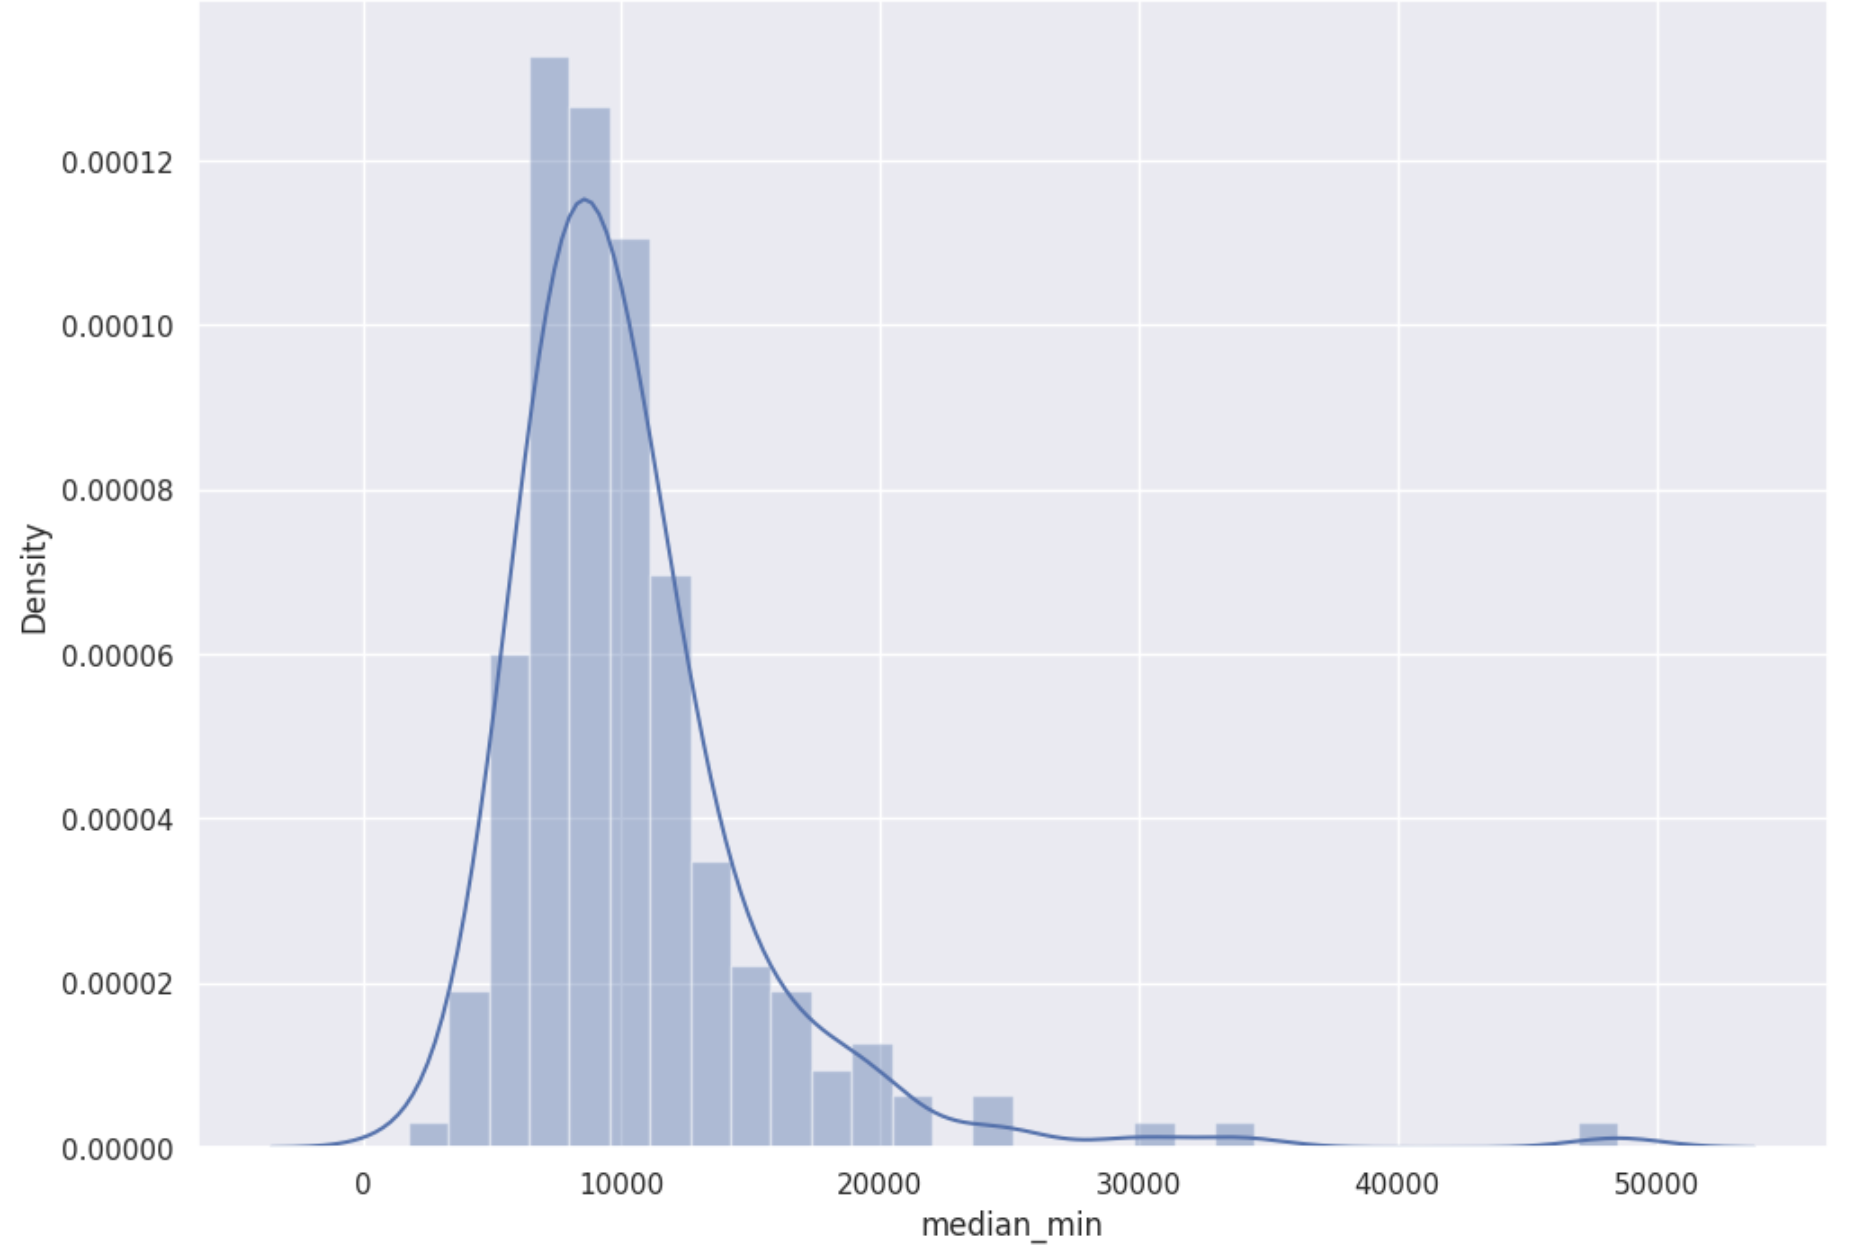
\includegraphics[width=1\textwidth, center]{verteilung_min.png}
    \caption[Verteilung von dem Preis Features \emph{median\_min}]{Verteilung von dem Preis Features \emph{median\_min}}
    \label{img:verteilung_min}
\end{figure}

Abbildung \ref{img:verteilung_min} zeigt, dass das Feature \emph{median\_min} eine Normalverteilung mit ein paar outlier aufweist. Eine Normalverteilung  sagt aus, dass die Verteilung mehr Daten um den Mittelwert herum aufweist. Die Datenverteilung nimmt ab, wenn sich vom Zentrum entfernt wird. Die resultierende Kurve ist symmetrisch zum Mittelwert und bildet eine glockenförmige Verteilung \cite{Shrishty.05.08.2021}.
\newline
\newline
Eine weitere interessante Information die noch aus dem Feature \emph{median\_min} gelesen werden kann, ist der Durchschnittliche Wert Region. Dazu soll der Datensatz nach der Region gruppiert werden und den Durchschnittlichen Wert ermittelt werden.
\newpage
\begin{figure}[h]
    \centering
    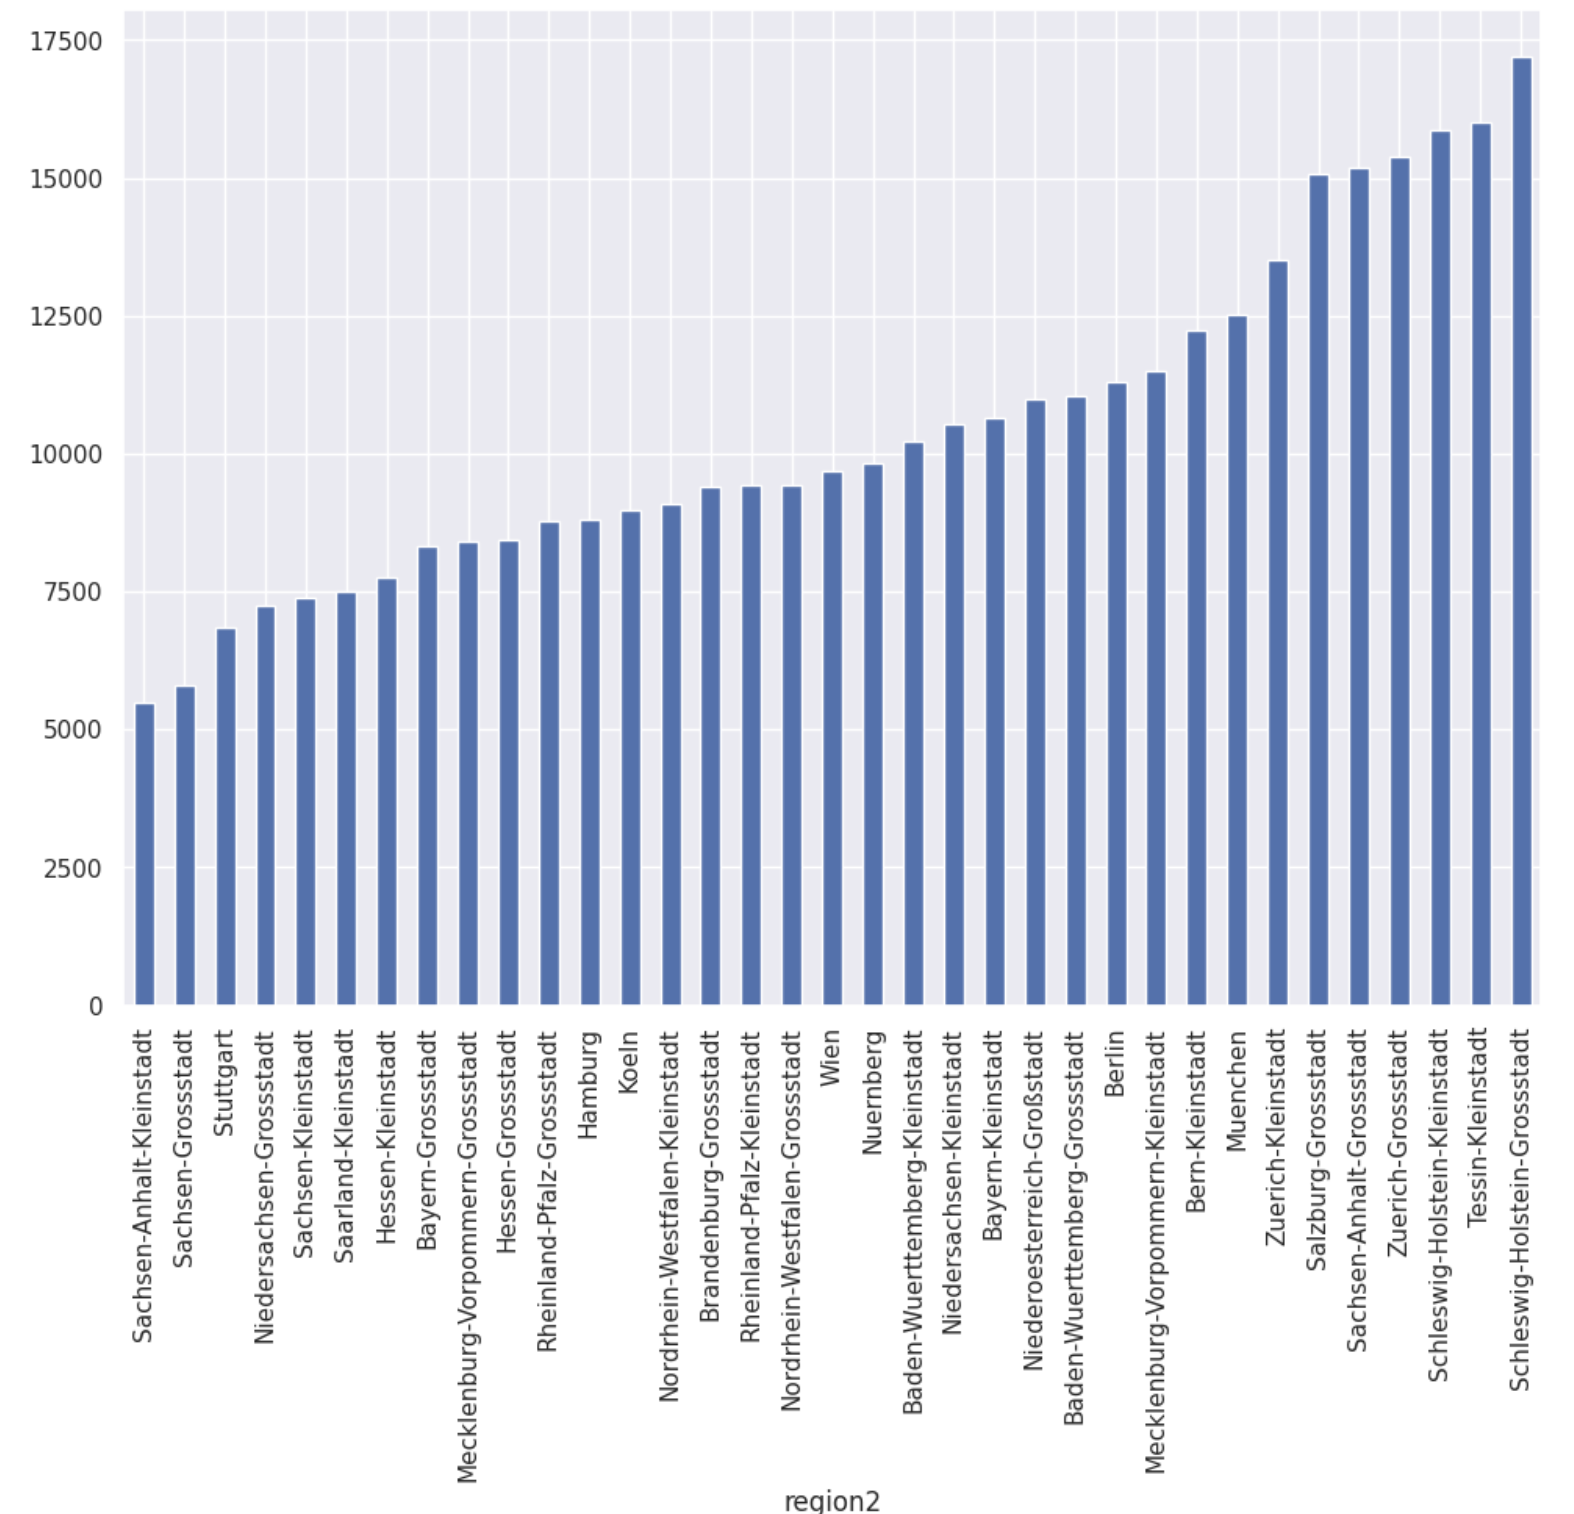
\includegraphics[width=0.6\textwidth, center]{avg_min_city.png}
    \caption[Durchschnittlicher minimal Preis pro Region]{Durchschnittlicher minimal Preis pro Region}
    \label{img:avg_min_city}
\end{figure}

Die Erkenntnis die aus der Abbildung \ref{img:avg_min_city} genommen werden kann, ist die, dass es einen deutlichen unterschied macht, in welcher Region das Hotel liegt wenn auf den Minimalen Median Preis des Hotel geschaut wird. Das gleich kann auch mit dem Maximalen Median Preis eines Hotels gemacht werden. Auch hier soll sich zunächst die Verteilung visualisiert werden:

\begin{figure}[h]
    \centering
    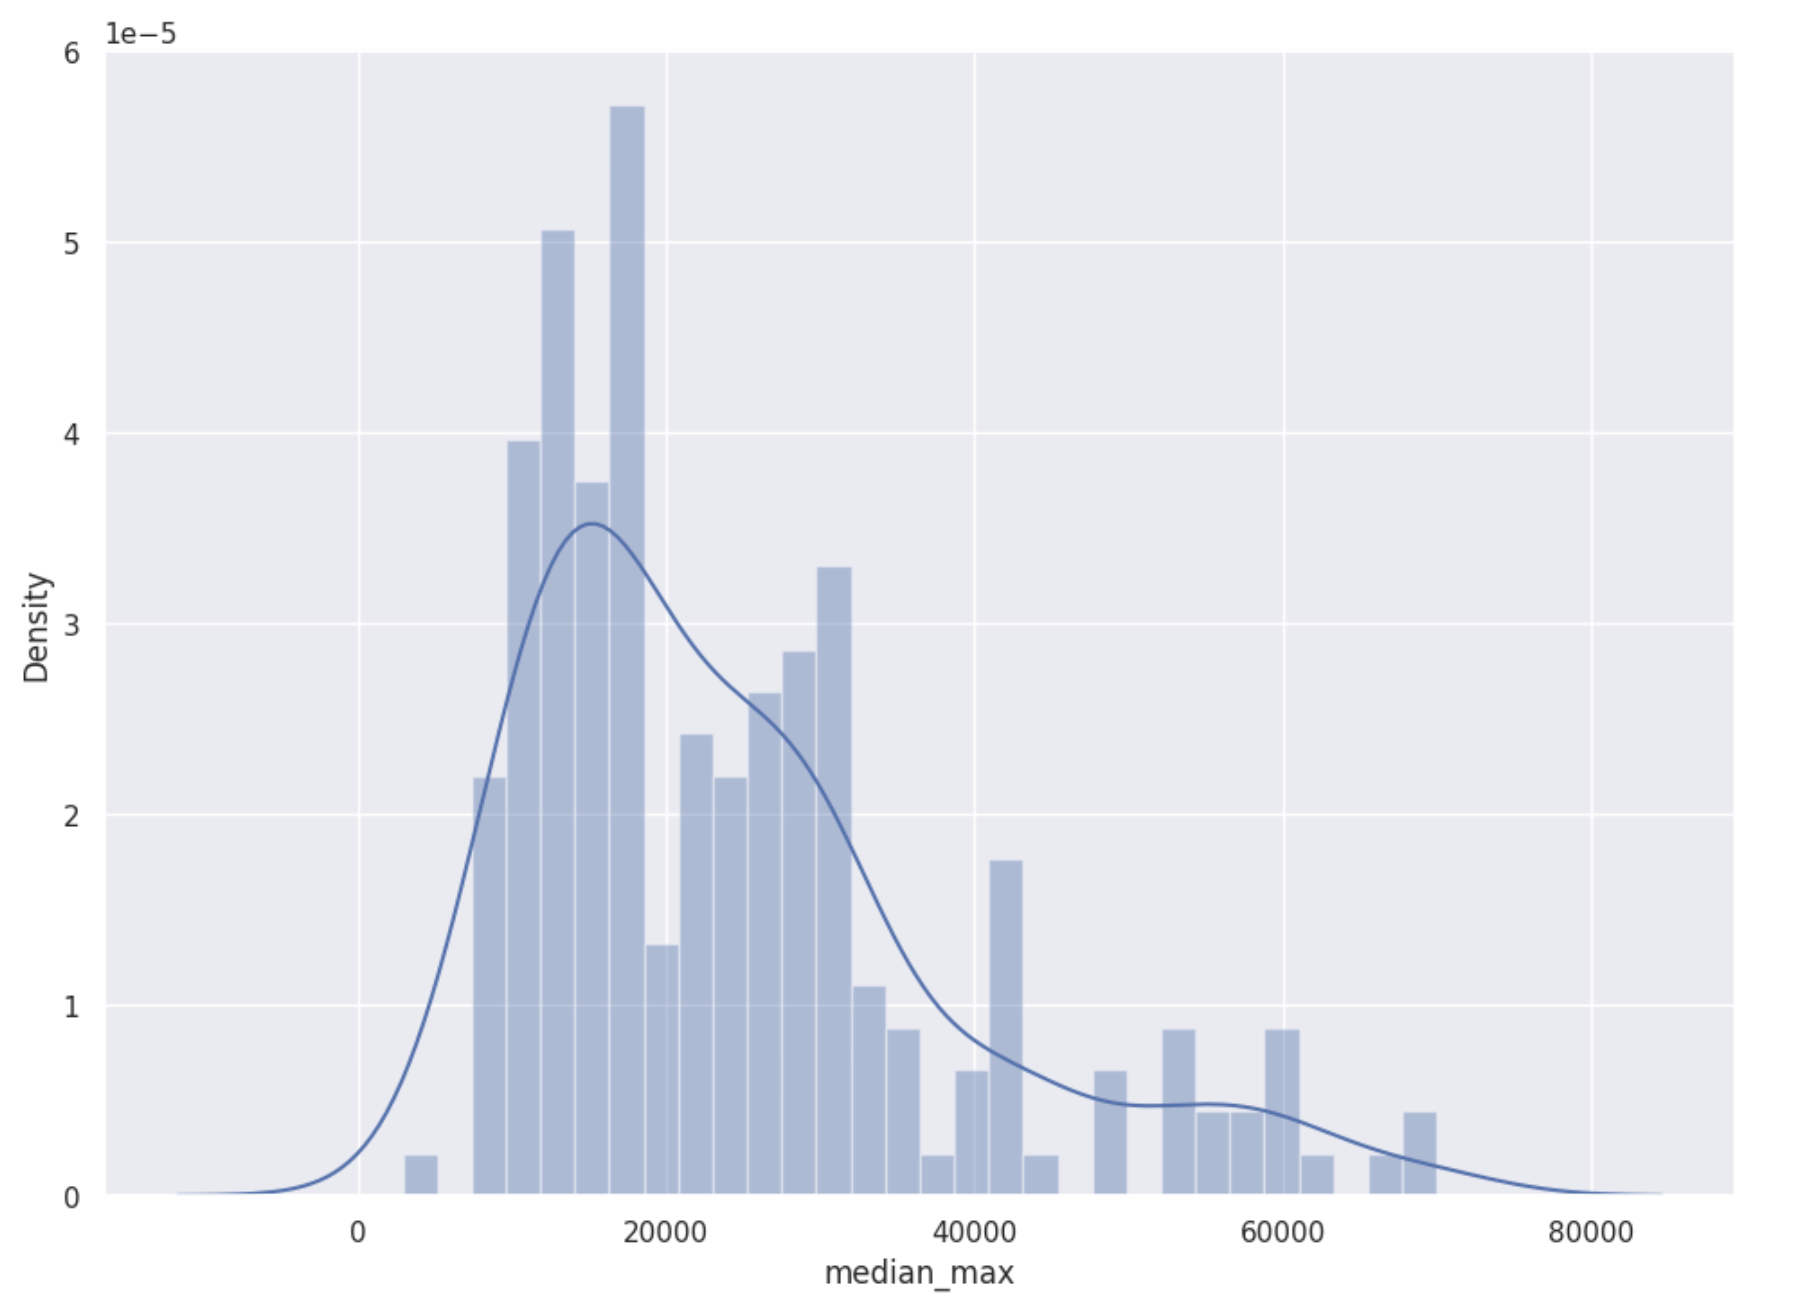
\includegraphics[width=0.6\textwidth, center]{verteilung_max.png}
    \caption[Verteilung von dem Preis Features \emph{median\_max}]{Verteilung von dem Preis Features \emph{median\_max}}
    \label{img:verteilung_max}
\end{figure}

Anders als bei dem Minimalen Median Preis, kann bei dem Maximalen Median Preis keine Normalverteilung erkannt werden. Hier wirken die Werte recht verstreut.

\begin{figure}[h]
    \centering
    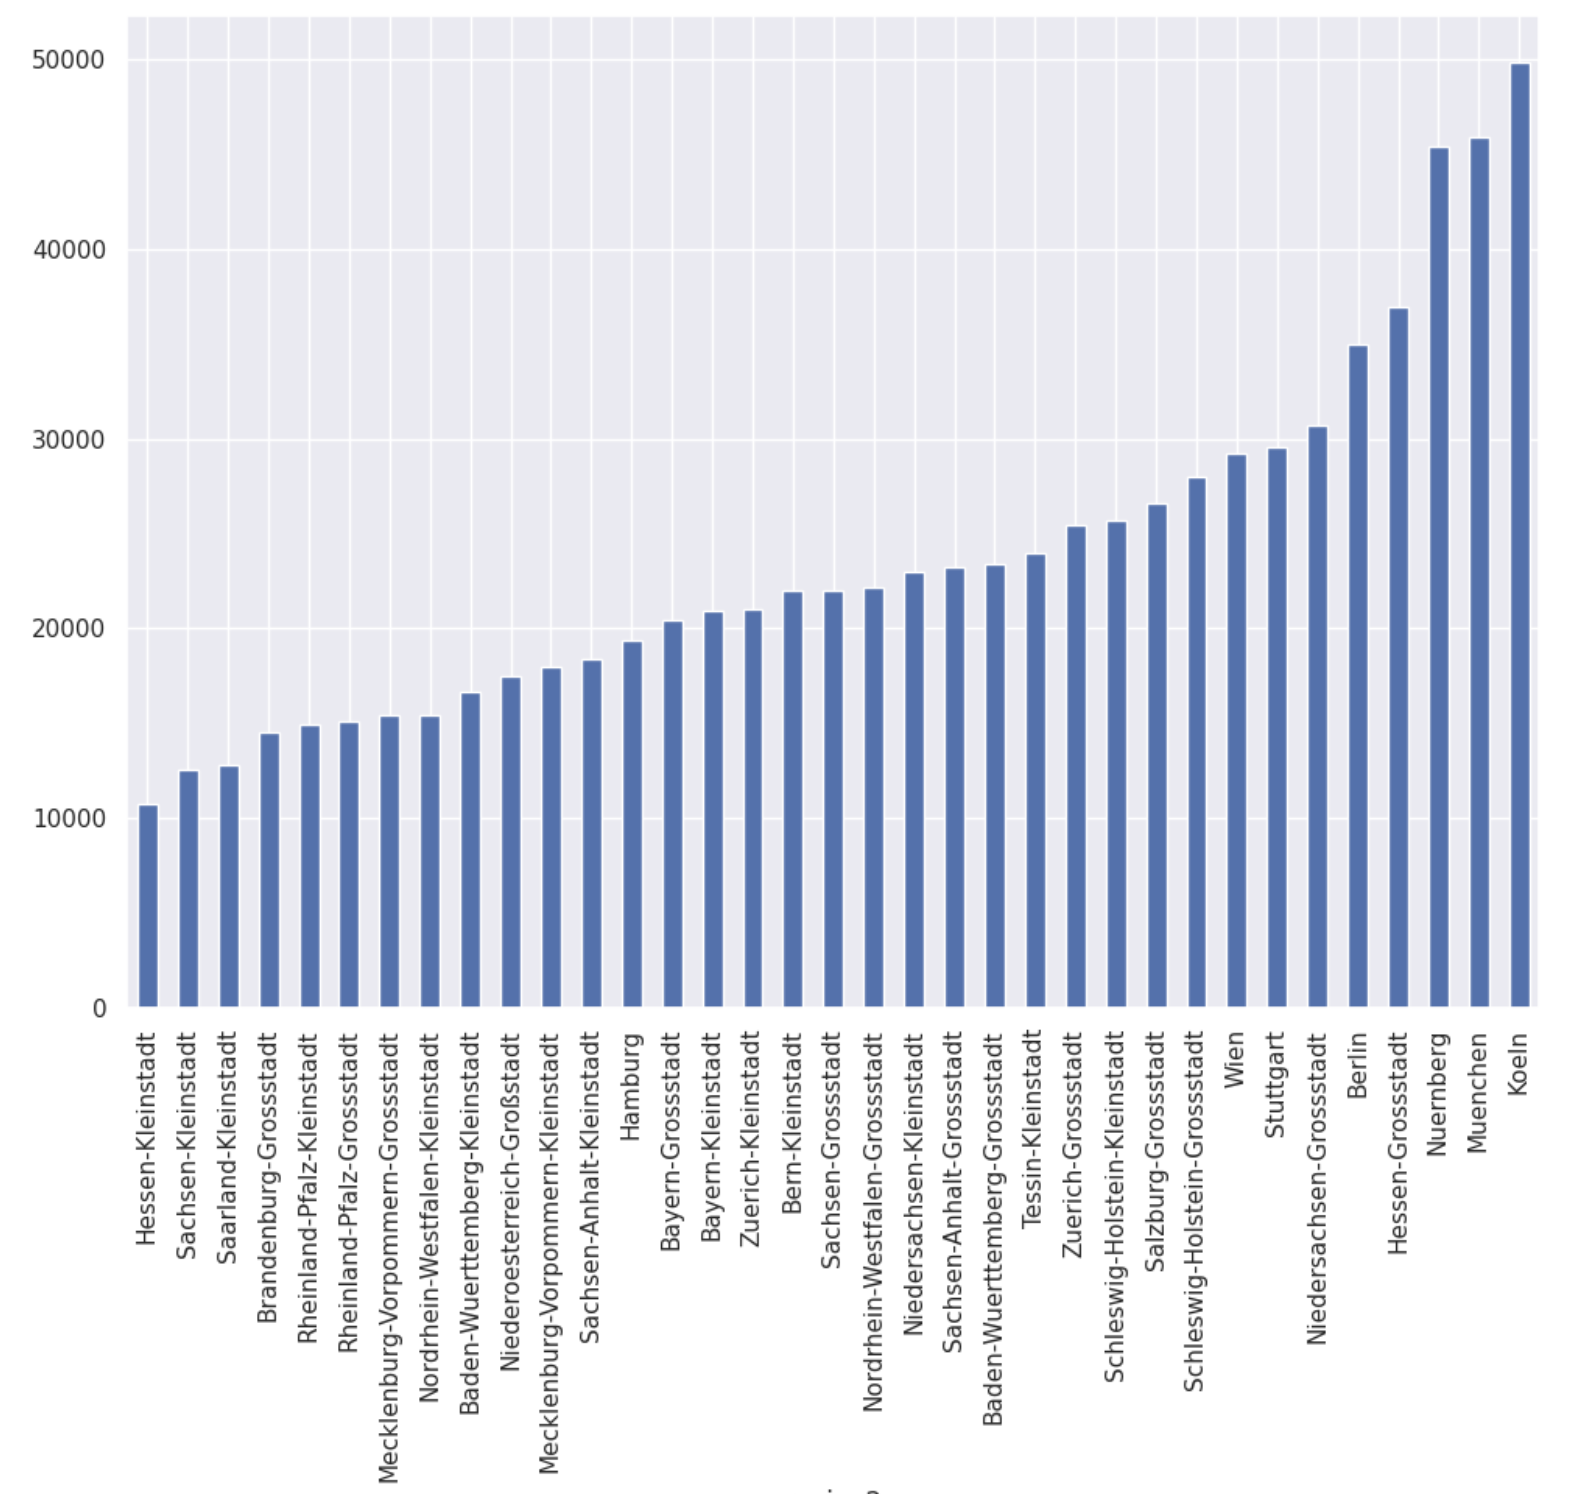
\includegraphics[width=1\textwidth, center]{avg_max_region.png}
    \caption[Durchschnittlicher maximal Preis pro Region]{Durchschnittlicher maximal Preis pro Region}
    \label{img:avg_max_city}
\end{figure}

Abbildung \ref{img:avg_max_city} zeigt, dass es auch deutliche Unterschiede bei den einzelnen Regionen gibt. Eine weitere interessante Erkenntnis ist die, dass es bei dem Maximalen Median Preis eher so ist, dass die Großstädte wie Köln und München eher zu einem höheren Maximalen Preis tendieren.

\subsubsection{Hotelart Feature}
Die Hotelart bildet einen essenziellen Bestandteil, um umfassende Einblicke in die Charakteristiken eines Hotels zu gewinnen. Sie liefert nicht nur Informationen über den Zweck und die Ausrichtung der Unterkunft, sondern ermöglicht auch eine präzise Identifikation der Zielgruppe, die das Hotel anspricht \cite{User.20.01.2024}. Die Zielgruppe eines Hotels ist zudem eine wertvolle Information wenn es darum geht Preise für das Hotel zu gestalten, zumindest ist so die Annahme. Auch in diesem Fall kann wieder nach der Hotelart gruppiert werden und jeweils der Minimale und Maximale durchschnittliche Preis angezeigt werden.

\begin{figure}[h]
    \centering
    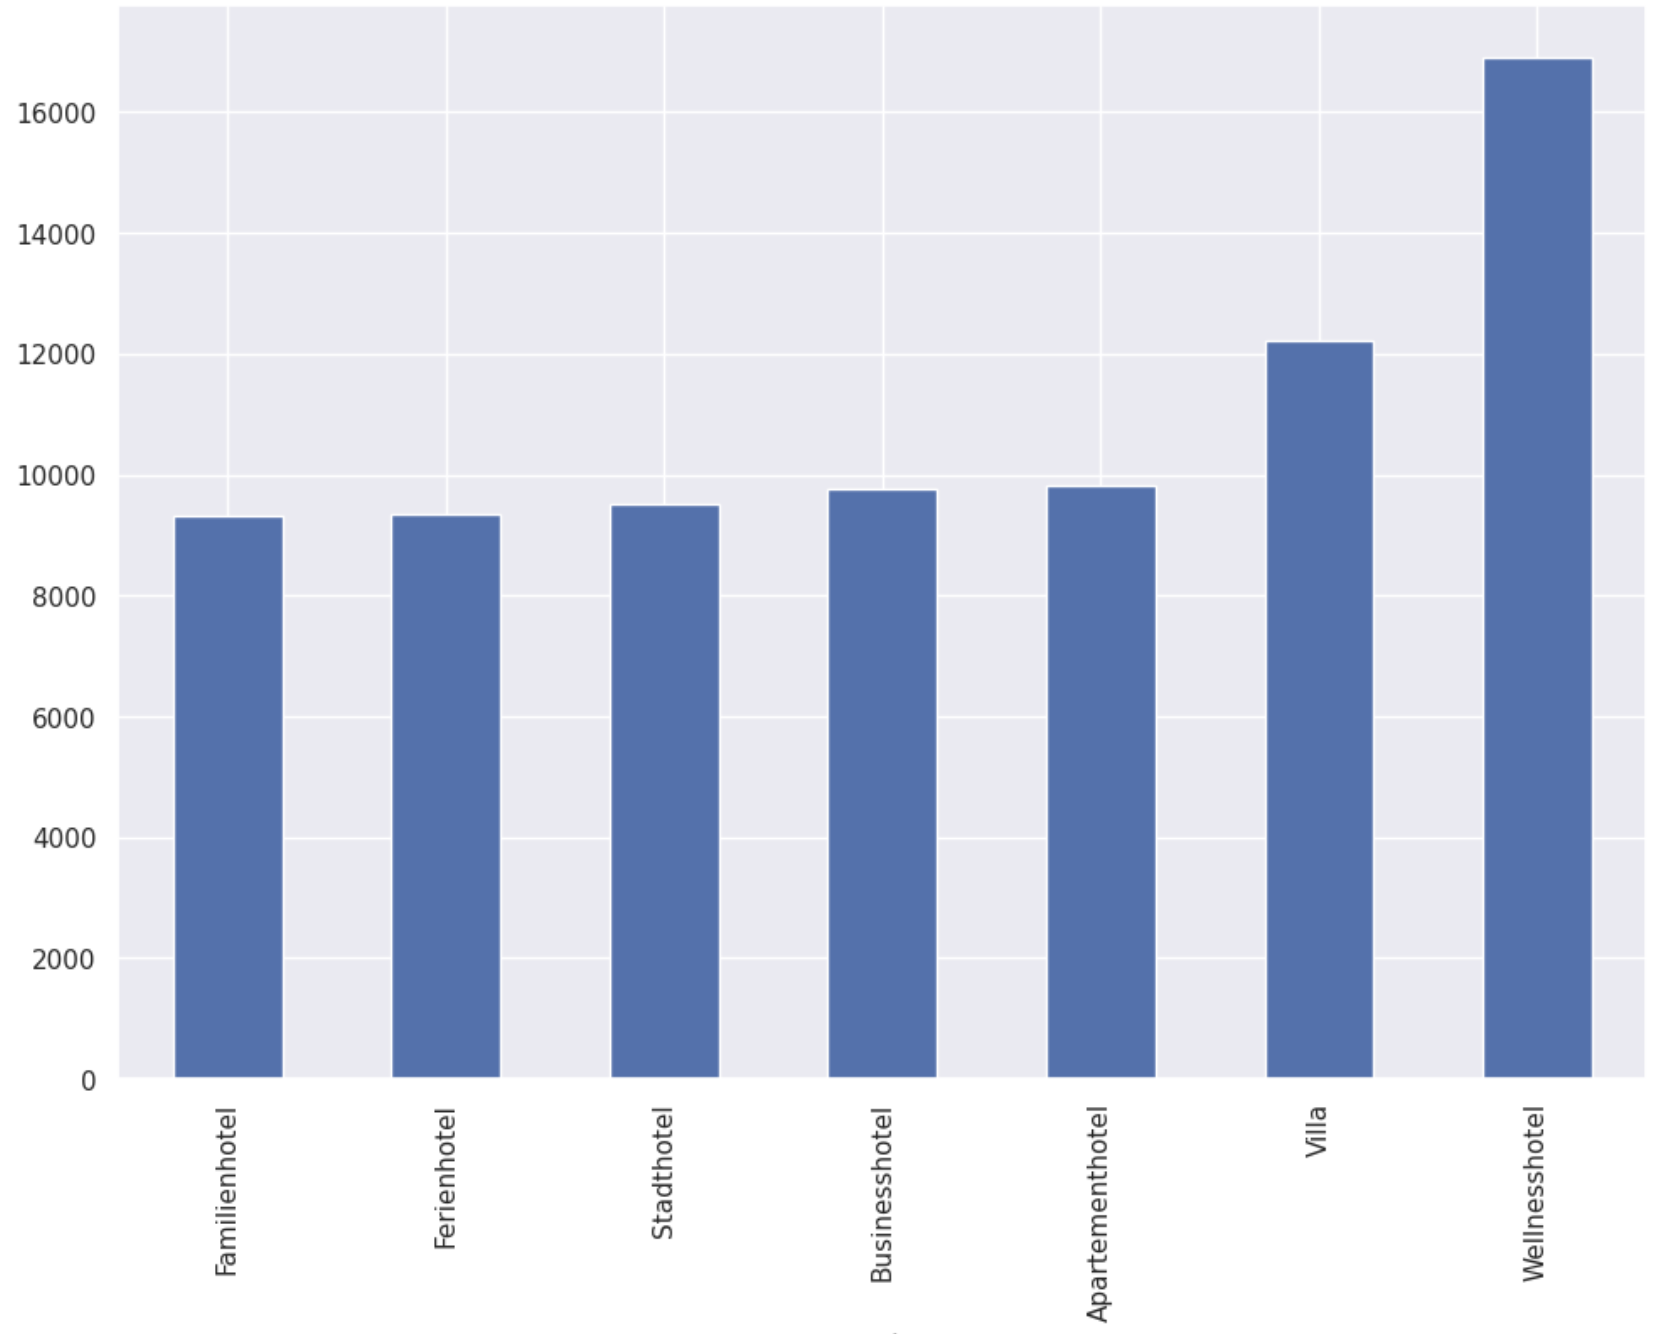
\includegraphics[width=0.6\textwidth, center]{avg_min_art.png}
    \caption[Durchschnittlicher minimal Preis pro Hotelart]{Durchschnittlicher minimal Preis pro Hotelart}
    \label{img:avg_min_art}
\end{figure}

\begin{figure}[h]
    \centering
    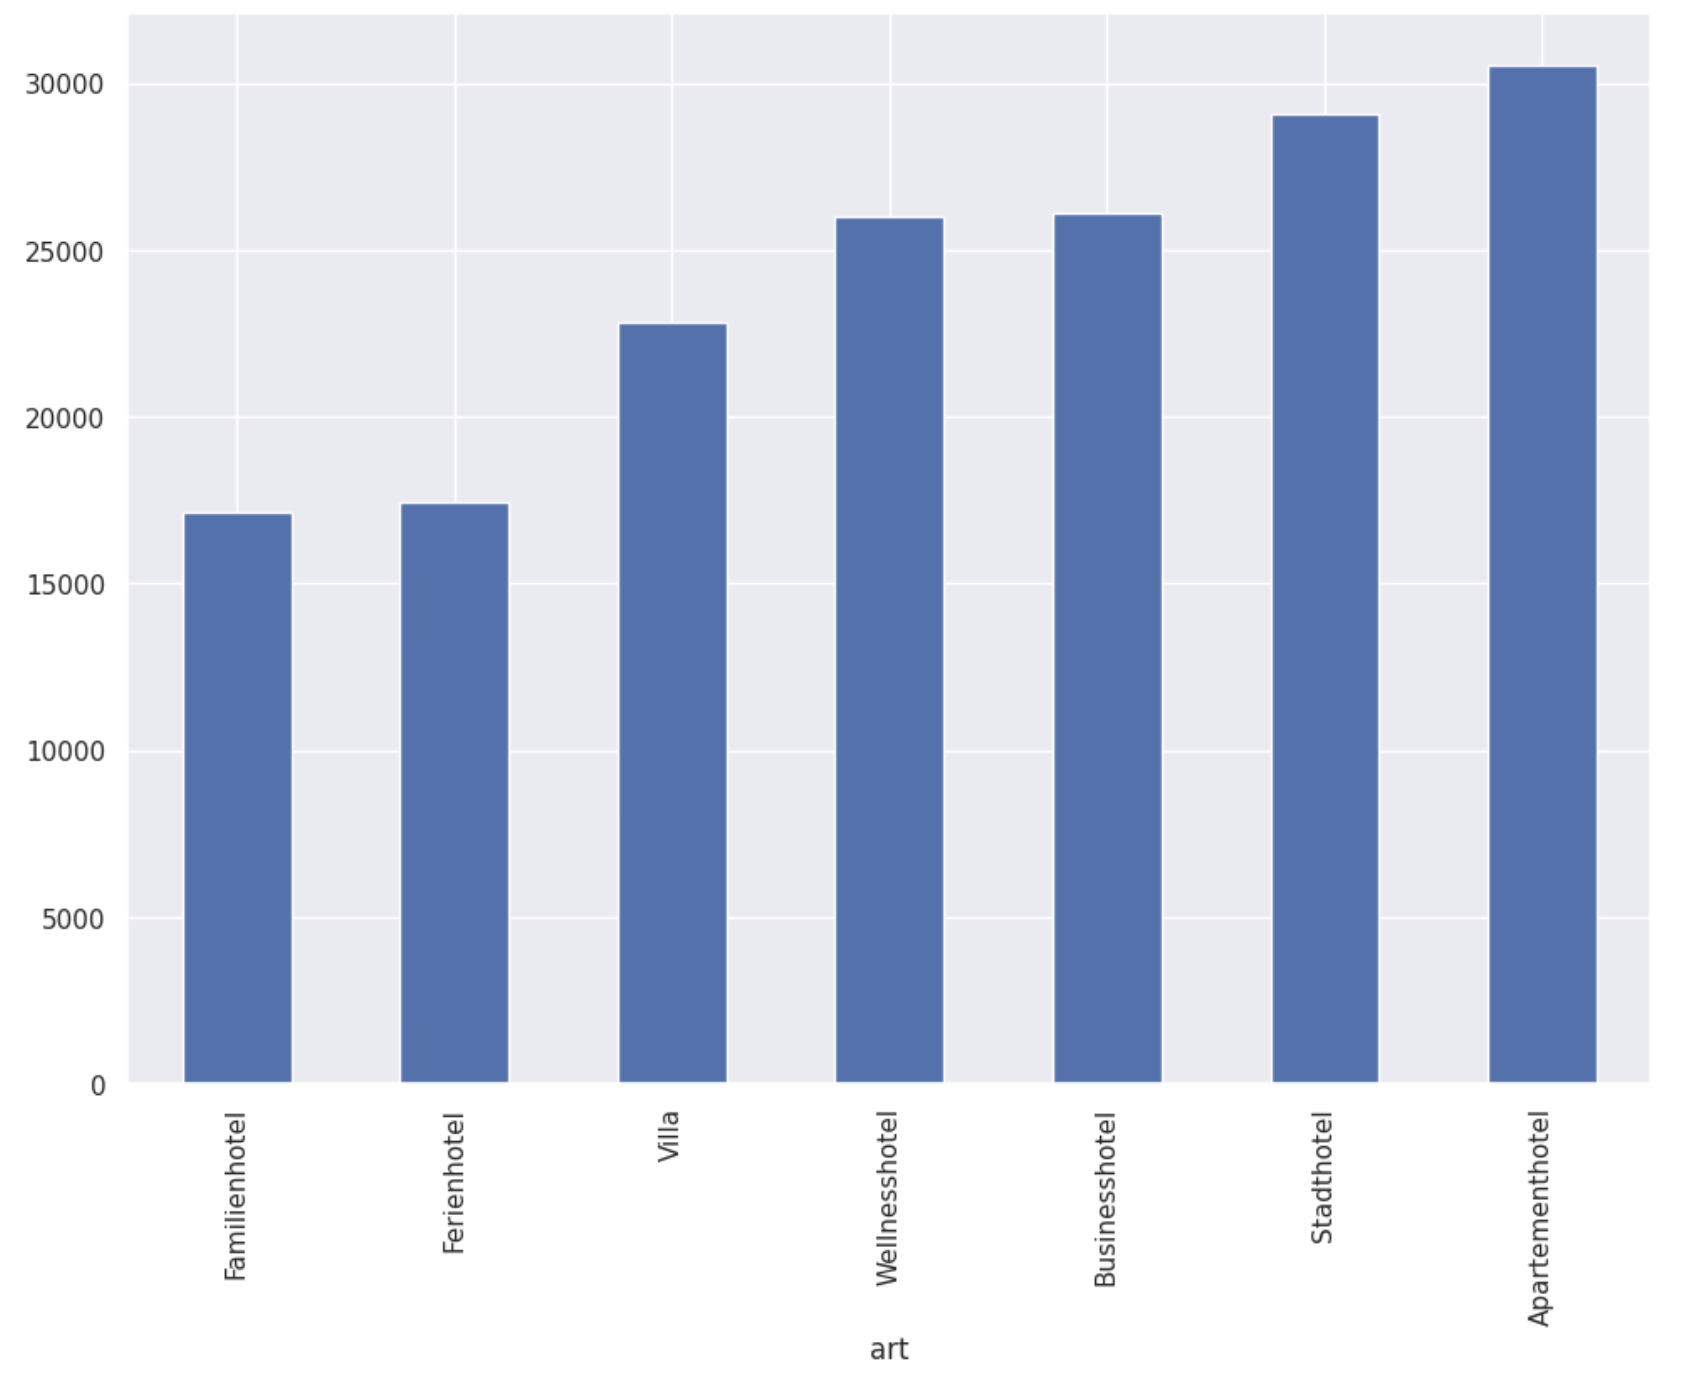
\includegraphics[width=0.6\textwidth, center]{avg_max_art.png}
    \caption[Durchschnittlicher maximal Preis pro Hotelart]{Durchschnittlicher maximal Preis pro Hotelart}
    \label{img:avg_max_art}
\end{figure}

Anhand von den zwei Abbildungen \ref{img:avg_min_art} und \ref{img:avg_max_art} zeigt sich, dass tatsächlich einen unterschied bei den Preisen auf die Hotelart bezogen gibt. Zudem zeigt sich, dass die zwei Hotelarten \emph{Ferienhotel} und \emph{Familienhotel} in beiden Fällen die gleiche Information wiedergibt und somit auch zu \emph{Ferienhotel} zusammengefasst werden kann. Zudem könnten anhand von \emph{median\_min} noch weitere Hotelarten zusammengefasst werden, jedoch wenn beide Informationen zusammen betrachtet werden, so bleibt es lediglich bei \emph{Ferienhotel} und \emph{Familienhotel}.

\subsubsection{Zimmer Features}
Die letzten zwei Features innerhalb des Datensatzes sind die Features \emph{area\_count} und \emph{areatype\_count} welche die Größe des jeweiligen Hotels repräsentieren. Die Frage die sich hier also stellt ist, ob das Preisverhältnis in irgendeiner Art mit der Größe des Hotels zusammenhängen kann. Hierzu soll zunächst auch erstmal die Verteilung der Zimmeranzahl angeschaut werden:

\begin{figure}[h]
    \centering
    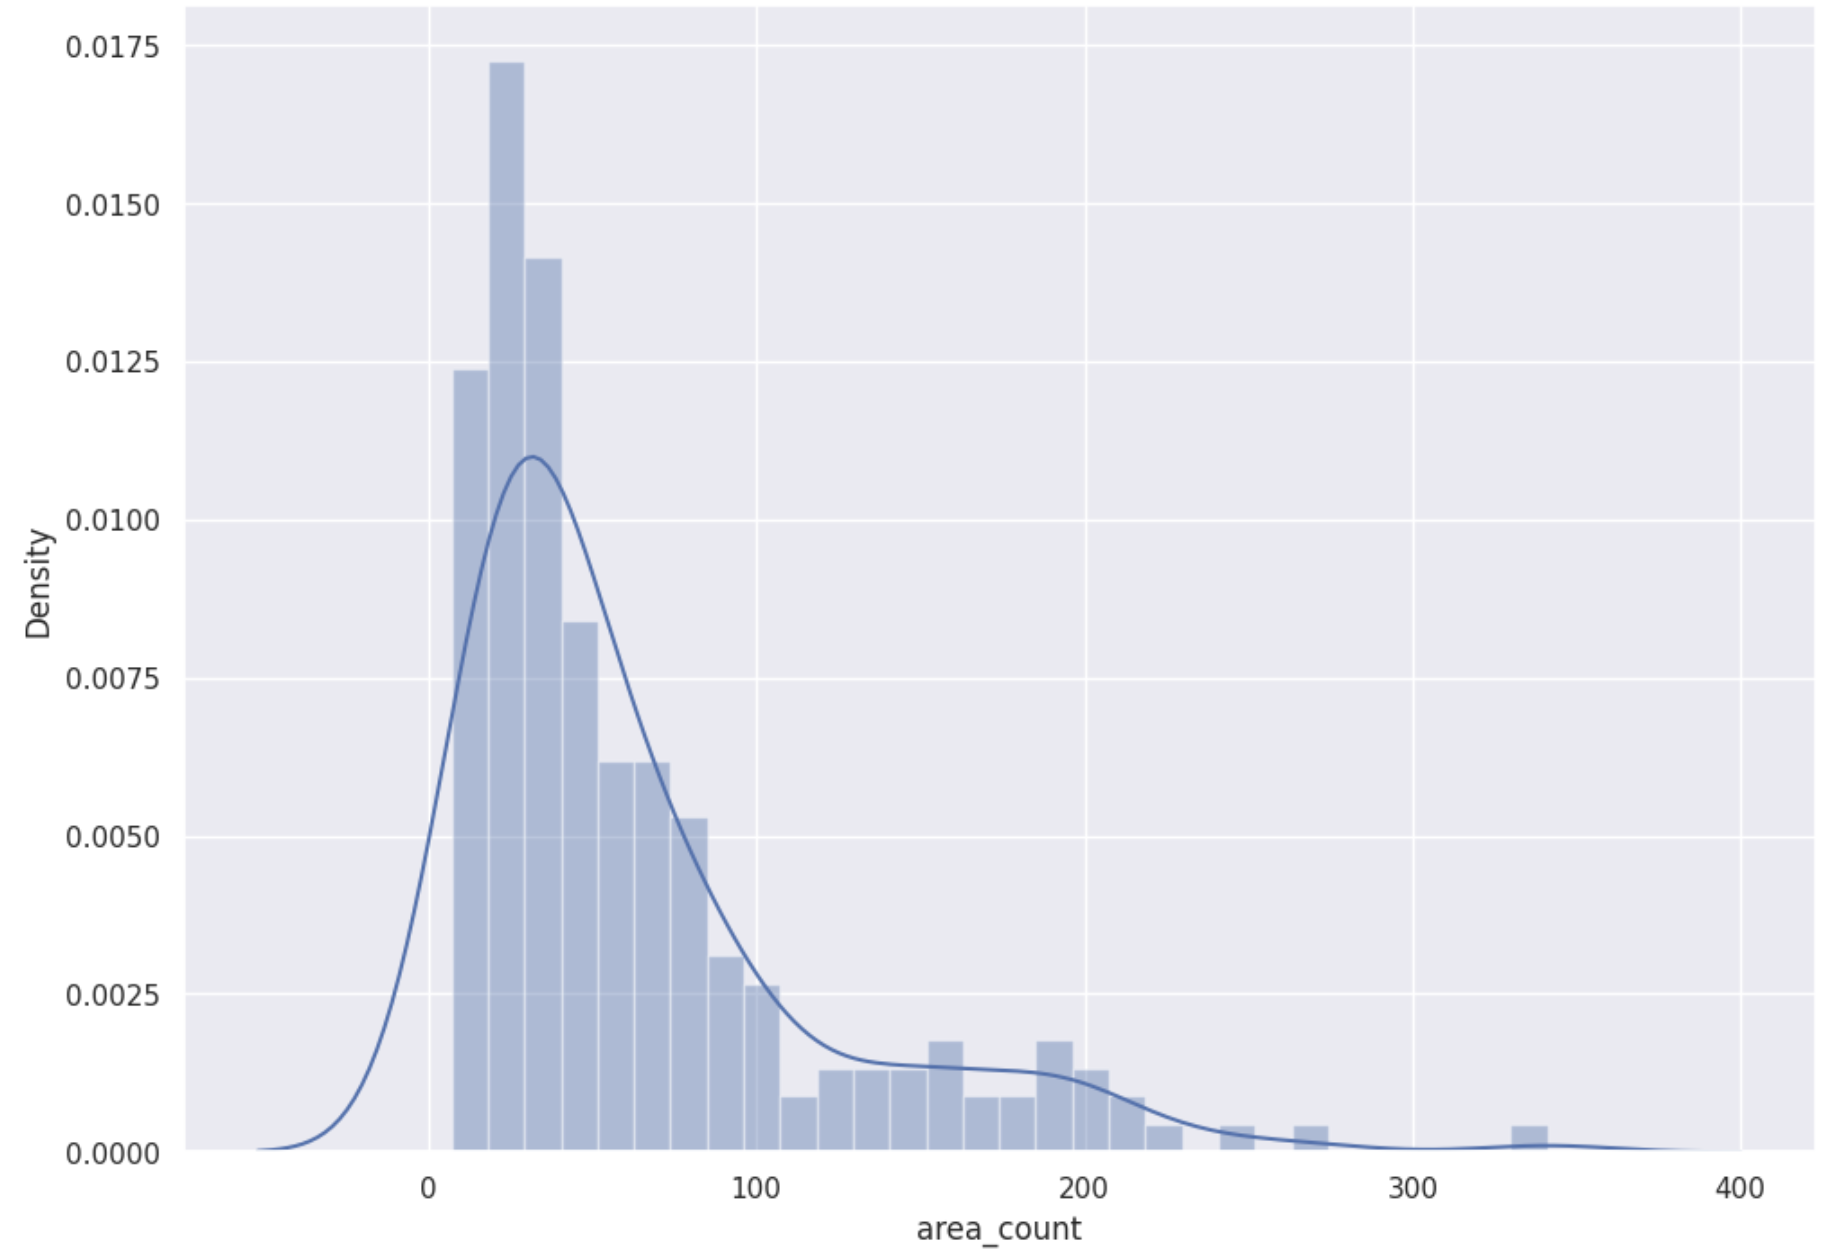
\includegraphics[width=0.6\textwidth, center]{verteilung_area_count.png}
    \caption[Verteilung nach Zimmeranzahl]{Verteilung nach Zimmeranzahl}
    \label{img:verteilung_area_count}
\end{figure}

Die Verteilung zeigt, dass auch recht ausgeprägt ist und nur im Ansatz einer Normalverteilung gleicht. Des Weiteren soll nach der Anzahl der Zimmer gruppiert werden um zu überprüfen wie oft jeder Anzahl vorkommt:

\begin{figure}[h]
    \centering
    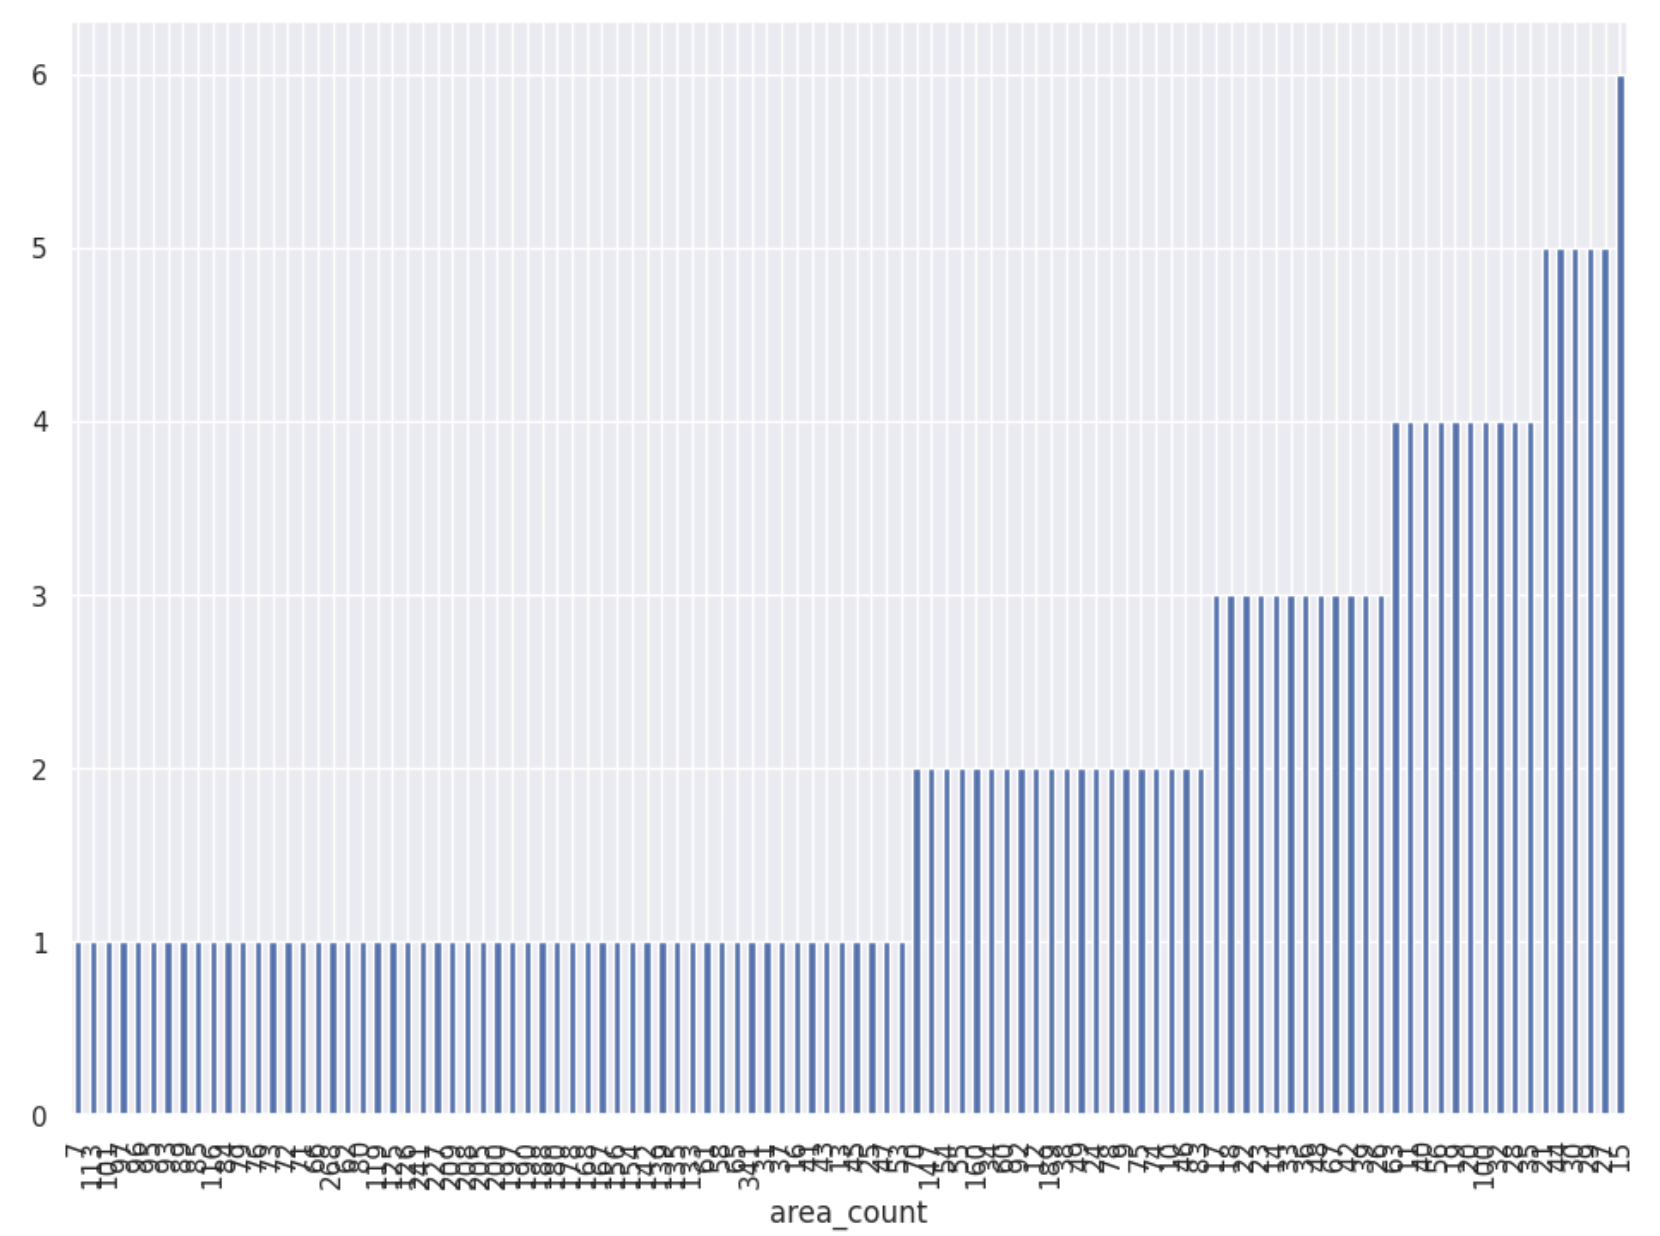
\includegraphics[width=0.6\textwidth, center]{group_area_count.png}
    \caption[Häufigkeit der Zimmeranzahl im Datensatz]{Häufigkeit der Zimmeranzahl im Datensatz}
    \label{img:haufigkeit_area_count}
\end{figure}
Abbildung \ref{img:haufigkeit_area_count} hat gezeigt, dass das Feature \emph{area\_count} zu ausgeprägt ist. Aufgrund dessen, dass das Feature zu ausgeprägt ist und keine Idee vorhanden ist, wie dieses Feature umformuliert werden könnte, wurde beschlossen \emph{area\_count} und \emph{areatype\_count} aus dem Datensatz zu entfernen.
\newline
\newline
Der finale Datensatz welcher für das Modell benutzt werden soll, sieht wie folgt aus:

\begin{figure}[h]
    \centering
    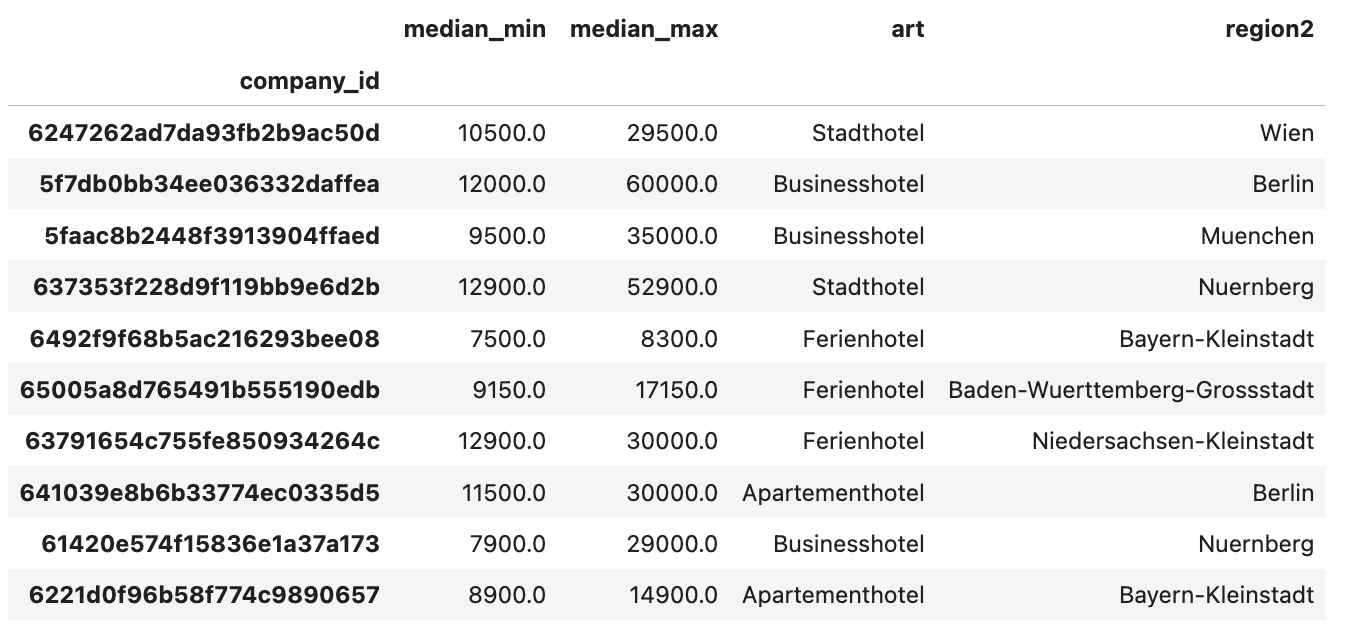
\includegraphics[width=1\textwidth, center]{all_features_4.png}
    \caption[Finaler Datensatz für das Modell]{Finaler Datensatz für das Modell}
    \label{img:all_features_4}
\end{figure}
\subsection{Evaluation der Ähnlichen Hotels}
\label{subsec:Evaluation_1}
Der vorliegende Datensatz ist nun verfügbar, und grundsätzlich kann die Modellierung fortgesetzt werden. Allerdings stellt sich die Frage, ob die identifizierten Hotels tatsächlich ähnlich zum ursprünglichen Hotel sind. Es ist von entscheidender Bedeutung, nachzuweisen, dass die ausgewählten Hotels auf irgendeine Weise miteinander vergleichbar sind. Aus diesem Grund wird im nachfolgenden Abschnitt ein Mechanismus entwickelt, um die Ähnlichkeit der Hotels zu überprüfen und zu gewährleisten.
\newline
\newline
Angesichts des angestrebten Ziels, nämlich der dynamischen Generierung von Preisen, wurde zunächst in Erwägung gezogen, die Preise der einzelnen Hotels zu vergleichen. Zu diesem Zweck wurde initial ein \emph{Dataframe} erstellt, das sämtliche gültigen Hotels sowie ihre Preisinformationen für einen bestimmten Zeitraum umfasst.
\newpage
\begin{figure}[h]
    \centering
    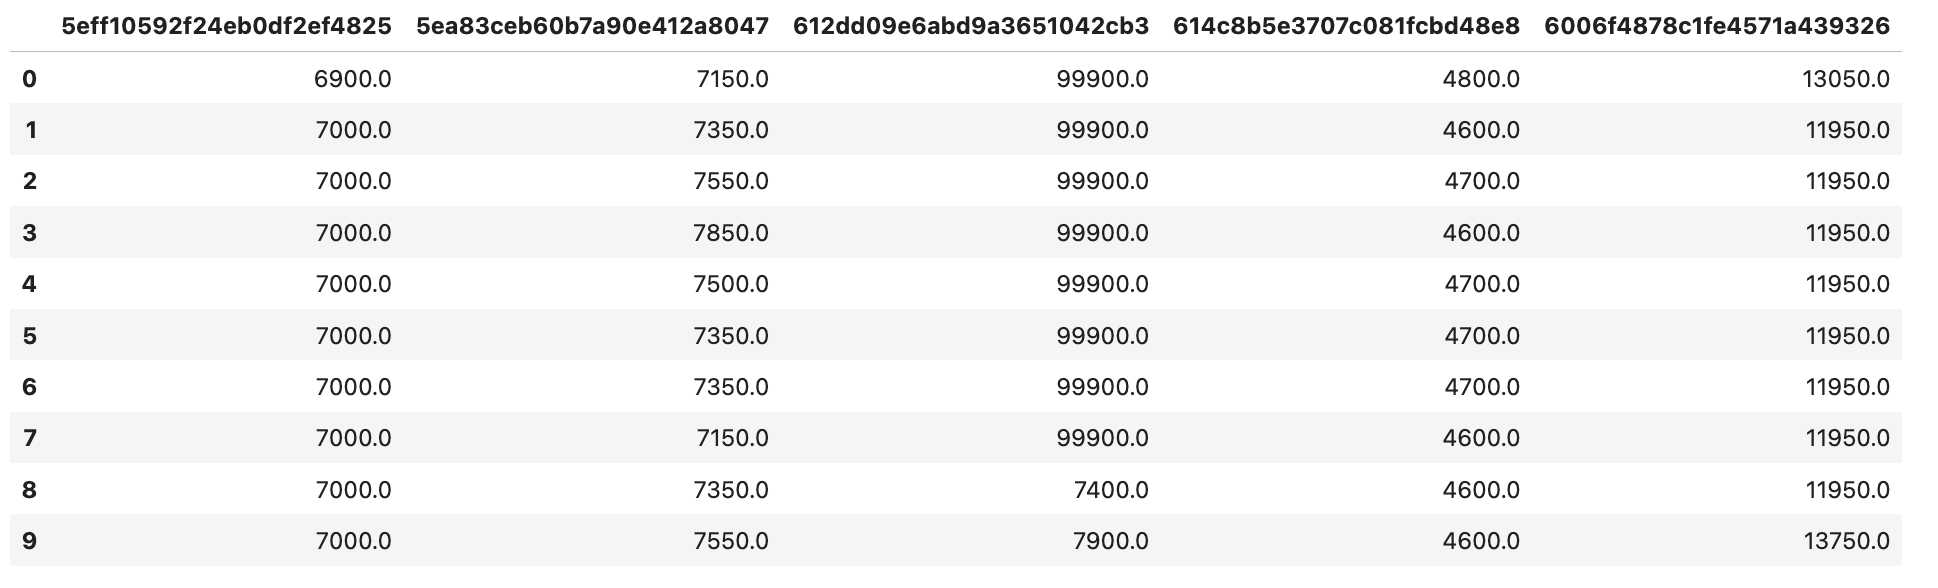
\includegraphics[width=0.9\textwidth, center]{all_prices.png}
    \caption[Preise von allen Hotels für das Jahr 2022]{Preise von allen Hotels für das Jahr 2022}
    \label{img:all_prices}
\end{figure}

Abbildung \ref{img:all_prices} zeigt einen exemplarischen Auszug aus dem DataFrame. Zudem wurde anhand diesem DataFrame noch die dazugehörige Korrelationsmatrix erstellt. Die Korrelationsmatrix ist dafür da um zusammenhänge zwischen den Vektoren zu finden. Dabei beschreibt ein Wert nahe 1 einen hohen positiven Zusammenhang der zwei Vektoren und ein Wert nahe -1 einen hohen negativen Zusammenhang der zwei Vektoren. Ein Korrelationswert gegen 0 beschreibt beschreibt keinerlei Zusammenhang der Vektoren \cite{Team.03.05.2020}. Die Vermutung ist es, dass wenn die Preise von 2 Hotels korrelieren und die Preise sich überschneiden, so werden dass ähnliche Hotels sein. 
\newline
\newline
Diese Vermutung soll dementsprechend mit einigen Hotels getestet werden:
\begin{figure}[h]
    \centering
    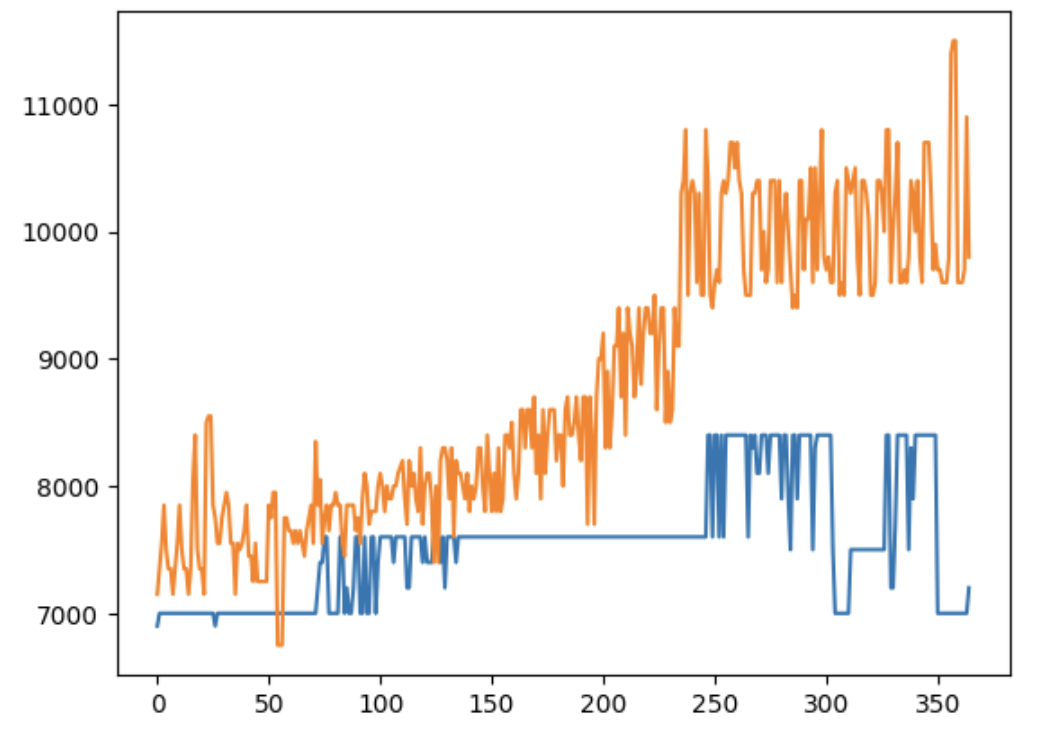
\includegraphics[width=0.9\textwidth, center]{preise_zwei_hotels.png}
    \caption[Visualisierung der Preise zweier Hotels]{Visualisierung der Preise zweier Hotels}
    \label{img:preise_zwei_hotels}
\end{figure}

\begin{figure}[h]
    \centering
    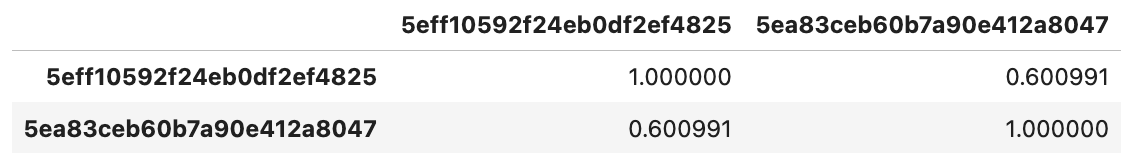
\includegraphics[width=1\textwidth, center]{corr_values_ex.png}
    \caption[Korrelationswerte der zwei Hotels]{Korrelationswerte der zwei Hotels}
    \label{img:corr_values_ex}
\end{figure}

Abbildung \ref{img:preise_zwei_hotels} illustriert den Preisverlauf von zwei Hotels im Jahr 2022, während Abbildung \ref{img:corr_values_ex} die Korrelation zwischen diesen beiden Hotels zeigt. Der festgestellte Korrelationswert von 0,6 erweist sich als bemerkenswert, insbesondere vor dem Hintergrund, dass die Preise in Abbildung \ref{img:preise_zwei_hotels} beträchtlich voneinander abweichen. Infolgedessen wurde die Überlegung angestellt, die Preise zu skalieren und daraufhin miteinander zu vergleichen. Entscheidend für ähnliche Hotels ist lediglich die Tendenz wie sich die Preise verhalten. 
\newline
\newline
Werden die Preise nun Skaliert ändert sich an der Korrelation nichts und die Skalierten Preise sehen nun wie folgt aus:

\begin{figure}[h]
    \centering
    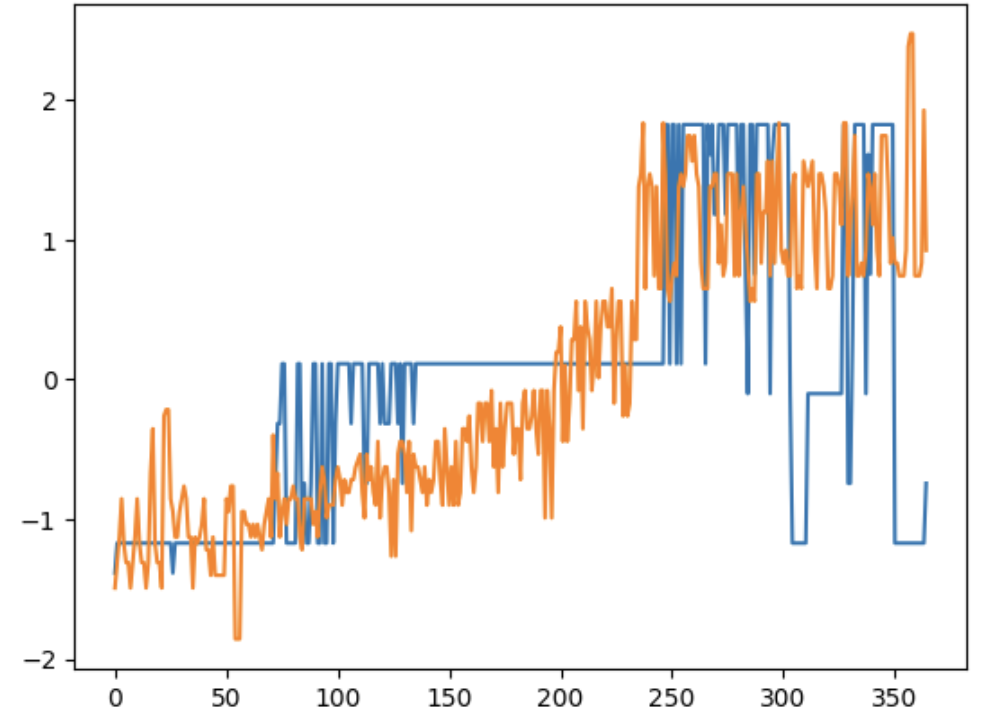
\includegraphics[width=1\textwidth, center]{scaled_preise_zwei_hotels.png}
    \caption[Visualisierung der Skalierten Preise zweier Hotels]{Visualisierung der Skalierten Preise zweier Hotels}
    \label{img:scaled_preise_zwei_hotels}
\end{figure}

Eine zusätzliche Betrachtung ergab die Frage, ob ein ähnliches Muster nicht auch durch die Verwendung des RevPAR erzielt werden könnte. Die Verwendung des RevPAR-Werts erscheint in diesem Kontext sinnvoller als die ausschließliche Berücksichtigung der Zimmerpreise, da das nachfolgende Modell letztendlich darauf abzielt, den RevPAR-Wert vorherzusagen.
\newline
\newline
Im folgenden werden die gleichen zwei Hotels mit dem RevPAR-Wert verglichen:

\begin{figure}[h]
    \centering
    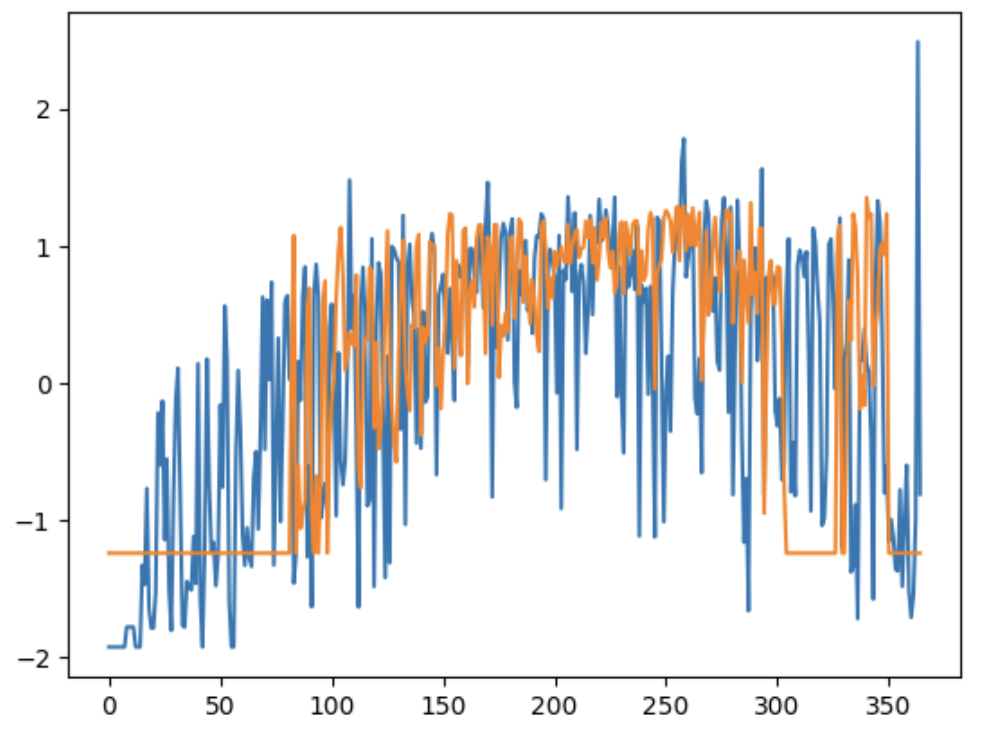
\includegraphics[width=1\textwidth, center]{scaled_revpar_zwei_hotels.png}
    \caption[Visualisierung der Skalierten RevPAR-Werte zweier Hotels]{Visualisierung der Skalierten RevPAR-Werte zweier Hotels}
    \label{img:scaled_revpar_zwei_hotels}
\end{figure}

\begin{figure}[h]
    \centering
    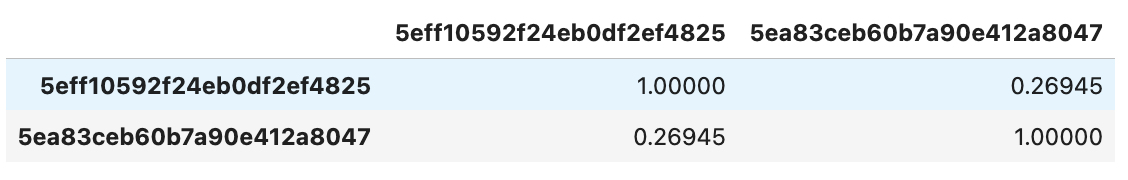
\includegraphics[width=1\textwidth, center]{corr_revpar_values_ex.png}
    \caption[Korrelationswerte der RevPAR-Werte zweier Hotels]{Korrelationswerte der RevPAR-Werte zweier Hotels}
    \label{img:corr_revpar_values_ex}
\end{figure}

Abbildung \ref{img:corr_revpar_values_ex} offenbarte einen abweichenden Korrelationswert im Vergleich zu demjenigen, der bei der Betrachtung der Preisentwicklung ermittelt wurde. Daraufhin wurde die Entscheidung getroffen, dass der Korrelationswert der RevPAR-Werte als aussagekräftiger betrachtet wird als derjenige der reinen Preisentwicklung. Infolgedessen wurde festgelegt, dass dieser Wert als Evaluation für die Ähnlichkeit zwischen den Hotels herangezogen wird.
\newline
\newline
Dieser Korrelationswert der RevPAR-Werte kann lediglich zur Evaluation der Modelle verwendet werden, da dieser Korrelationswert für ein Hotel nicht vorhanden ist. 